% ============================================================
%  Perricheno Platform — 25 IEEE Publication Figures
%  Compile with: pdflatex figures_ieee.tex
% ============================================================
\documentclass{article}
\usepackage[T1]{fontenc}
\usepackage[utf8]{inputenc}
\usepackage{tikz}
\usetikzlibrary{
  arrows.meta, positioning, shapes.geometric, shapes.multipart,
  fit, backgrounds, decorations.pathreplacing, decorations.markings,
  calc, matrix, mindmap, trees, patterns, chains
}
\usepackage{xcolor}
\usepackage{geometry}
\usepackage{amsmath}
\geometry{a4paper, margin=1.8cm}

% ── Palette ──────────────────────────────────────────────────────────────
\definecolor{CB}{RGB}{31,119,180}   % blue
\definecolor{CO}{RGB}{255,127,14}   % orange
\definecolor{CG}{RGB}{44,160,44}    % green
\definecolor{CR}{RGB}{214,39,40}    % red
\definecolor{CP}{RGB}{148,103,189}  % purple
\definecolor{CT}{RGB}{23,190,207}   % teal
\definecolor{CY}{RGB}{188,189,34}   % olive
\definecolor{LB}{RGB}{174,199,232}  % light blue
\definecolor{LO}{RGB}{255,187,120}  % light orange
\definecolor{LG}{RGB}{152,223,138}  % light green
\definecolor{LR}{RGB}{255,152,150}  % light red
\definecolor{LP}{RGB}{197,176,213}  % light purple
\definecolor{LT}{RGB}{158,218,229}  % light teal
\definecolor{LGr}{RGB}{225,225,225} % light gray
\definecolor{DG}{RGB}{50,50,50}     % dark gray
\definecolor{Cbrown}{RGB}{140,86,75}
\definecolor{Lcbrown}{RGB}{196,156,148}

\begin{document}

% ╔══════════════════════════════════════════════════════════════════════════╗
% ║  FIG 1 — Six-Stage LLM Pipeline                                         ║
% ╚══════════════════════════════════════════════════════════════════════════╝
\begin{figure}[h!]
\centering
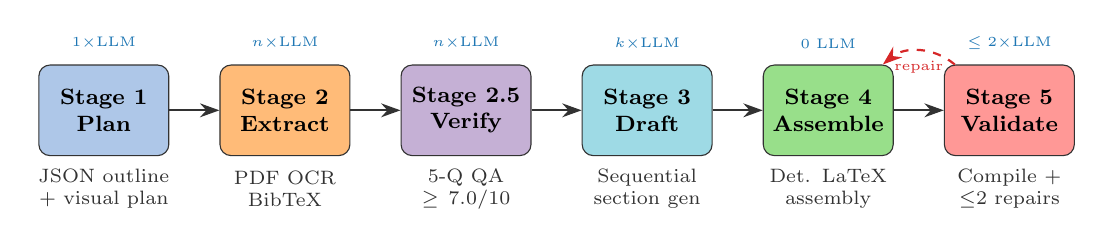
\begin{tikzpicture}[
  stg/.style={draw=DG, fill=#1, rounded corners=4pt,
              minimum width=1.65cm, minimum height=1.15cm,
              align=center, font=\footnotesize\bfseries},
  arr/.style={-{Stealth[length=7pt,width=5pt]}, thick, draw=DG},
  lbl/.style={font=\scriptsize, text=DG, align=center, text width=1.7cm},
  tok/.style={font=\tiny, text=CB}
]
\node[stg=LB]  (s1)  at (0,0)     {Stage 1\\Plan};
\node[stg=LO]  (s2)  at (2.3,0)   {Stage 2\\Extract};
\node[stg=LP]  (s25) at (4.6,0)   {Stage 2.5\\Verify};
\node[stg=LT]  (s3)  at (6.9,0)   {Stage 3\\Draft};
\node[stg=LG]  (s4)  at (9.2,0)   {Stage 4\\Assemble};
\node[stg=LR]  (s5)  at (11.5,0)  {Stage 5\\Validate};

\draw[arr] (s1)--(s2); \draw[arr] (s2)--(s25);
\draw[arr] (s25)--(s3); \draw[arr] (s3)--(s4); \draw[arr] (s4)--(s5);

% Repair back-edge
\draw[arr, draw=CR, dashed, bend right=40]
  (s5) to node[below, font=\tiny, text=CR]{repair} (s4);

\node[lbl] at (0,-1.0)   {JSON outline\\+ visual plan};
\node[lbl] at (2.3,-1.0) {PDF OCR\\BibTeX};
\node[lbl] at (4.6,-1.0) {5-Q QA\\\(\geq 7.0/10\)};
\node[lbl] at (6.9,-1.0) {Sequential\\section gen};
\node[lbl] at (9.2,-1.0) {Det. LaTeX\\assembly};
\node[lbl] at (11.5,-1.0){Compile +\\\(\leq\)2 repairs};

\node[tok] at (0,0.85)    {\(1{\times}\)LLM};
\node[tok] at (2.3,0.85)  {\(n{\times}\)LLM};
\node[tok] at (4.6,0.85)  {\(n{\times}\)LLM};
\node[tok] at (6.9,0.85)  {\(k{\times}\)LLM};
\node[tok] at (9.2,0.85)  {0 LLM};
\node[tok] at (11.5,0.85) {\(\leq 2{\times}\)LLM};
\end{tikzpicture}
\caption{Six-stage document generation pipeline. Arrows show data flow;
         dashed arrow shows LaTeX repair feedback. Token annotations indicate
         LLM invocations per stage (\(n\)=uploads, \(k\)=sections).}
\label{fig:pipeline}
\end{figure}

% ╔══════════════════════════════════════════════════════════════════════════╗
% ║  FIG 2 — Platform Layered Architecture                                  ║
% ╚══════════════════════════════════════════════════════════════════════════╝
\begin{figure}[h!]
\centering
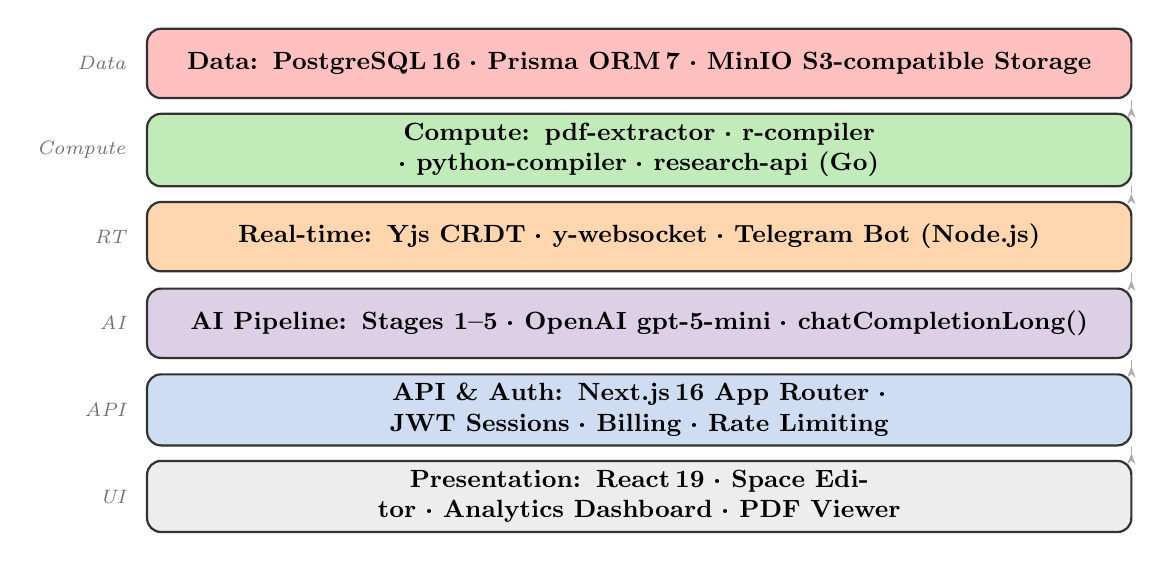
\begin{tikzpicture}[
  layer/.style={draw=DG, thick, rounded corners=5pt,
                minimum width=12.5cm, minimum height=0.88cm,
                align=center, font=\small\bfseries, text width=12cm},
  badge/.style={font=\scriptsize\itshape, text=DG!70, anchor=east}
]
\node[layer,fill=LGr!60]  (L1) at (0,0.00) {Presentation: React\,19 · Space Editor · Analytics Dashboard · PDF Viewer};
\node[layer,fill=LB!60]   (L2) at (0,1.10) {API \& Auth: Next.js\,16 App Router · JWT Sessions · Billing · Rate Limiting};
\node[layer,fill=LP!60]   (L3) at (0,2.20) {AI Pipeline: Stages 1--5 · OpenAI gpt-5-mini · chatCompletionLong()};
\node[layer,fill=LO!60]   (L4) at (0,3.30) {Real-time: Yjs CRDT · y-websocket · Telegram Bot (Node.js)};
\node[layer,fill=LG!60]   (L5) at (0,4.40) {Compute: pdf-extractor · r-compiler · python-compiler · research-api (Go)};
\node[layer,fill=LR!60]   (L6) at (0,5.50) {Data: PostgreSQL\,16 · Prisma ORM\,7 · MinIO S3-compatible Storage};

\node[badge] at (-6.4,0.00)  {UI};
\node[badge] at (-6.4,1.10)  {API};
\node[badge] at (-6.4,2.20)  {AI};
\node[badge] at (-6.4,3.30)  {RT};
\node[badge] at (-6.4,4.40)  {Compute};
\node[badge] at (-6.4,5.50)  {Data};

% Vertical connectors on right side
\foreach \y in {0.55,1.65,2.75,3.85,4.95}
  \draw[draw=DG!40, -{Stealth[length=4pt]}, thin] (6.25,\y)--(6.25,\y+0.0);
\end{tikzpicture}
\caption{Perricheno six-layer architecture. Each layer isolates a distinct
         concern: data, compute, AI, real-time, API, and presentation.}
\label{fig:architecture}
\end{figure}

% ╔══════════════════════════════════════════════════════════════════════════╗
% ║  FIG 3 — Confidence-Gated RAG Decision Flow                             ║
% ╚══════════════════════════════════════════════════════════════════════════╝
\begin{figure}[h!]
\centering
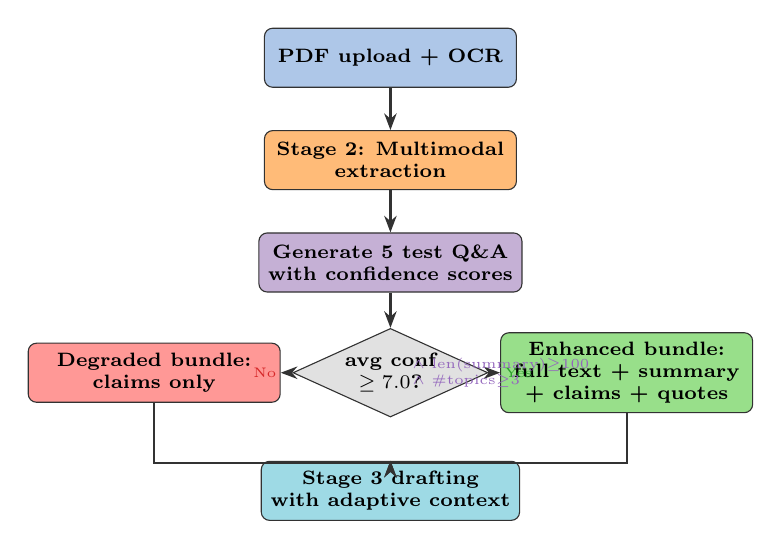
\begin{tikzpicture}[
  box/.style={draw=DG, rounded corners=3pt, fill=#1,
              minimum width=3.2cm, minimum height=0.75cm,
              align=center, font=\scriptsize\bfseries},
  dia/.style={draw=DG, diamond, aspect=2.2, fill=#1,
              align=center, font=\scriptsize\bfseries, inner sep=1pt},
  arr/.style={-{Stealth[length=6pt]}, thick, draw=DG},
  yes/.style={font=\tiny, text=CG, midway, anchor=west},
  no/.style={font=\tiny, text=CR, midway, anchor=east}
]
% Nodes (vertical layout)
\node[box=LB]  (pdf)   at (0,0)    {PDF upload + OCR};
\node[box=LO]  (ext)   at (0,-1.3) {Stage 2: Multimodal\\extraction};
\node[box=LP]  (gen)   at (0,-2.6) {Generate 5 test Q\&A\\with confidence scores};
\node[dia=LGr] (thr)   at (0,-4.0) {avg conf\\ $\geq 7.0$?};
\node[box=LG]  (enh)   at (3.0,-4.0){Enhanced bundle:\\full text + summary\\+ claims + quotes};
\node[box=LR]  (deg)   at (-3.0,-4.0){Degraded bundle:\\claims only};
\node[box=LT]  (s3)    at (0,-5.5) {Stage 3 drafting\\with adaptive context};

\draw[arr] (pdf)--(ext);
\draw[arr] (ext)--(gen);
\draw[arr] (gen)--(thr);
\draw[arr] (thr)--node[yes]{Yes}(enh);
\draw[arr] (thr)--node[no]{No}(deg);
\draw[arr] (enh)|-(0,-5.15)--(s3);
\draw[arr] (deg)|-(0,-5.15)--(s3);

% Threshold annotation
\node[font=\tiny, text=CP, align=left, anchor=west] at (0.15,-4.0)
  {$\land$ len(summary)$\geq$100\\$\land$ \#topics$\geq$3};
\end{tikzpicture}
\caption{Confidence-gated RAG verification (Stage\,2.5). An LLM-as-evaluator
         protocol with multi-criteria thresholds selects between two reference
         bundle quality tiers for downstream drafting.}
\label{fig:rag}
\end{figure}

% ╔══════════════════════════════════════════════════════════════════════════╗
% ║  FIG 4 — TikZ Blueprint Compile-Validate-Repair Cycle                   ║
% ╚══════════════════════════════════════════════════════════════════════════╝
\begin{figure}[h!]
\centering
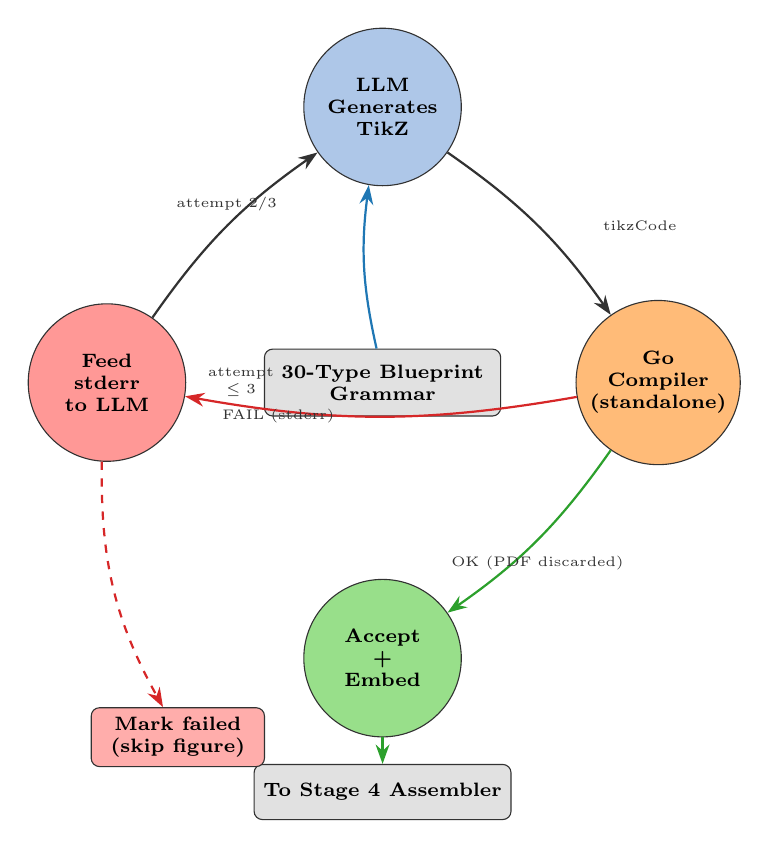
\begin{tikzpicture}[
  circ/.style={draw=DG, circle, fill=#1, minimum size=2.0cm,
               align=center, font=\scriptsize\bfseries, inner sep=2pt},
  rect/.style={draw=DG, rounded corners=3pt, fill=#1,
               minimum width=2.6cm, minimum height=0.7cm,
               align=center, font=\scriptsize\bfseries},
  arr/.style={-{Stealth[length=7pt,width=5pt]}, thick, draw=DG},
  lbl/.style={font=\tiny, text=DG, align=center, text width=2.2cm}
]
% Central hub
\node[rect=LGr, minimum width=3cm, minimum height=0.85cm]
  (bp) at (0,0) {30-Type Blueprint\\Grammar};

% States on circle
\node[circ=LB]  (gen)  at (90:3.5)   {LLM\\Generates\\TikZ};
\node[circ=LO]  (comp) at (0:3.5)    {Go\\Compiler\\(standalone)};
\node[circ=LG]  (ok)   at (270:3.5)  {Accept\\+\\Embed};
\node[circ=LR]  (rep)  at (180:3.5)  {Feed\\stderr\\to LLM};

% Arrows (clockwise)
\draw[arr, CB] (bp)  to[bend left=10]  (gen);
\draw[arr]     (gen) to[bend left=10]  node[lbl, right=2pt]{tikzCode} (comp);
\draw[arr, CG] (comp) to[bend left=10] node[lbl, below=2pt]{OK (PDF discarded)} (ok);
\draw[arr, CR] (comp) to[bend left=10] node[lbl, left=2pt]{FAIL (stderr)} (rep);
\draw[arr]     (rep) to[bend left=10]  node[lbl, above=2pt]{attempt 2/3} (gen);

% Attempt counter
\node[font=\tiny, text=DG, align=center] at (180:1.8)
  {attempt\\$\leq 3$};
% Final output
\node[rect=LGr, minimum width=2.5cm] (out) at (270:5.2) {To Stage 4 Assembler};
\draw[arr, CG] (ok)--(out);
\node[rect=LR!80, minimum width=2.2cm] (fail) at (240:5.2) {Mark failed\\(skip figure)};
\draw[arr, CR, dashed] (rep) to[bend right=15] (fail);
\end{tikzpicture}
\caption{Compile-validate-repair loop for TikZ diagram generation. The LaTeX
         compiler acts as a formal correctness oracle; stderr feeds back into
         the LLM for iterative self-repair (max 3 attempts).}
\label{fig:tikz-repair}
\end{figure}

% ╔══════════════════════════════════════════════════════════════════════════╗
% ║  FIG 5 — concurrentMap Worker Pool                                      ║
% ╚══════════════════════════════════════════════════════════════════════════╝
\begin{figure}[h!]
\centering
\begin{tikzpicture}[
  item/.style={draw=DG, fill=#1, rounded corners=2pt,
               minimum width=0.7cm, minimum height=0.45cm,
               font=\tiny\bfseries, align=center},
  worker/.style={draw=DG!60, fill=LGr, rounded corners=3pt,
                 minimum width=11.5cm, minimum height=0.65cm,
                 align=center, font=\scriptsize},
  hdr/.style={font=\scriptsize\bfseries, text=DG, anchor=west}
]
% Input queue
\node[hdr] at (-6.0, 3.0) {Input queue};
\foreach \i/\c in {1/LB, 2/LO, 3/LP, 4/LT, 5/LG, 6/LR, 7/LB, 8/LO} {
  \node[item=\c] at (-5.5+\i*0.85, 3.0) {\i};
}

% Workers
\node[hdr] at (-6.0, 1.8) {Worker 1};
\node[worker] (w1) at (0, 1.8) {};
\node[item=LB, minimum width=1.4cm] at (-4.5,1.8) {1};
\node[item=LT, minimum width=1.4cm] at (-2.9,1.8) {4};
\node[item=LR, minimum width=1.4cm] at (-1.3,1.8) {7};
\node[font=\tiny,text=DG] at (2.0,1.8) {(maxConcurrency=4)};

\node[hdr] at (-6.0, 1.0) {Worker 2};
\node[worker] at (0, 1.0) {};
\node[item=LO, minimum width=1.4cm] at (-4.5,1.0) {2};
\node[item=LG, minimum width=1.4cm] at (-2.9,1.0) {5};
\node[item=LO, minimum width=1.4cm] at (-1.3,1.0) {8};

\node[hdr] at (-6.0, 0.2) {Worker 3};
\node[worker] at (0, 0.2) {};
\node[item=LP, minimum width=1.4cm] at (-4.5,0.2) {3};
\node[item=LB, minimum width=1.4cm] at (-2.9,0.2) {6};

\node[hdr] at (-6.0,-0.6) {Worker 4};
\node[worker] at (0,-0.6) {};
\node[font=\tiny, text=DG!60, italic] at (-2.0,-0.6) {idle};

% Output (order-preserving)
\node[hdr] at (-6.0,-1.6) {Output (order-preserved)};
\foreach \i/\c in {1/LB, 2/LO, 3/LP, 4/LT, 5/LG, 6/LR, 7/LB, 8/LO} {
  \node[item=\c] at (-5.5+\i*0.85, -1.6) {\i};
}

% Time axis
\draw[-{Stealth}, draw=DG!50, thin] (-5.5,-2.2)--(5.5,-2.2)
  node[right, font=\tiny]{time};

% Brace: concurrency bound
\draw[decorate, decoration={brace,amplitude=5pt}, draw=DG!60]
  (-6.0,2.2)--(-6.0,-1.0)
  node[midway, left=7pt, font=\tiny\itshape, text=DG]{\rotatebox{90}{bounded concurrency}};
\end{tikzpicture}
\caption{\texttt{concurrentMap()} bounded worker pool: items dispatched to up
         to \(N\) concurrent workers; output array preserves input ordering
         regardless of completion order.}
\label{fig:concurrentmap}
\end{figure}

% ╔══════════════════════════════════════════════════════════════════════════╗
% ║  FIG 6 — chatCompletionLong Token Continuation                          ║
% ╚══════════════════════════════════════════════════════════════════════════╝
\begin{figure}[h!]
\centering
\begin{tikzpicture}[
  call/.style={draw=DG, fill=#1, rounded corners=3pt,
               minimum width=3.8cm, minimum height=0.65cm,
               align=center, font=\scriptsize\bfseries},
  resp/.style={draw=DG!50, dashed, fill=#1, rounded corners=3pt,
               minimum width=3.8cm, minimum height=0.65cm,
               align=center, font=\scriptsize},
  arr/.style={-{Stealth[length=5pt]}, thick, draw=DG},
  note/.style={font=\tiny, text=DG, align=left, text width=4.5cm, anchor=west}
]
\node[call=LB]  (c1) at (0, 0)   {Call 1: full prompt};
\node[resp=LO]  (r1) at (0,-1.2) {Response 1 — TRUNCATED\\finish\_reason: ``length''};
\node[call=LB]  (c2) at (0,-2.5) {Call 2: tail[−1500 chars]\\+ ``continue…''};
\node[resp=LO]  (r2) at (0,-3.7) {Response 2 — TRUNCATED};
\node[call=LB]  (c3) at (0,-5.0) {Call 3: tail[−1500 chars]\\+ ``continue…''};
\node[resp=LG]  (r3) at (0,-6.2) {Response 3 — COMPLETE\\finish\_reason: ``stop''};

\draw[arr] (c1)--(r1);
\draw[arr] (r1)--(c2);
\draw[arr] (c2)--(r2);
\draw[arr] (r2)--(c3);
\draw[arr] (c3)--(r3);

% Side notes
\node[note] at (2.2, 0)   {System + user prompt\\(section task)};
\node[note] at (2.2,-1.2) {Partial text; triggers\\continuation logic};
\node[note] at (2.2,-2.5) {Sliding 1 500-char\\context window};
\node[note] at (2.2,-6.2) {Concatenated:\\text 1 + text 2 + text 3};

% Token counter
\node[font=\tiny, text=CP, anchor=east] at (-2.2,-0.0) {tokens: $t_1$};
\node[font=\tiny, text=CP, anchor=east] at (-2.2,-2.5) {tokens: $t_2$};
\node[font=\tiny, text=CP, anchor=east] at (-2.2,-5.0) {tokens: $t_3$};
\node[font=\tiny, text=CB, anchor=east] at (-2.2,-6.8)
  {total: $\sum t_i \times 3 = $ billed chars};

\draw[decorate, decoration={brace, amplitude=5pt}, draw=DG!50]
  (2.0,-0.3)--(2.0,-6.5)
  node[midway, right=8pt, font=\tiny\itshape, text=DG]
    {max 3 iterations};
\end{tikzpicture}
\caption{\texttt{chatCompletionLong()} auto-continuation mechanism. Truncated
         responses trigger subsequent calls with a sliding 1\,500-character
         tail window, enabling generation beyond single-call token limits.}
\label{fig:continuation}
\end{figure}

% ╔══════════════════════════════════════════════════════════════════════════╗
% ║  FIG 7 — 30-Type Visual Taxonomy (Partial Radial)                       ║
% ╚══════════════════════════════════════════════════════════════════════════╝
\begin{figure}[h!]
\centering
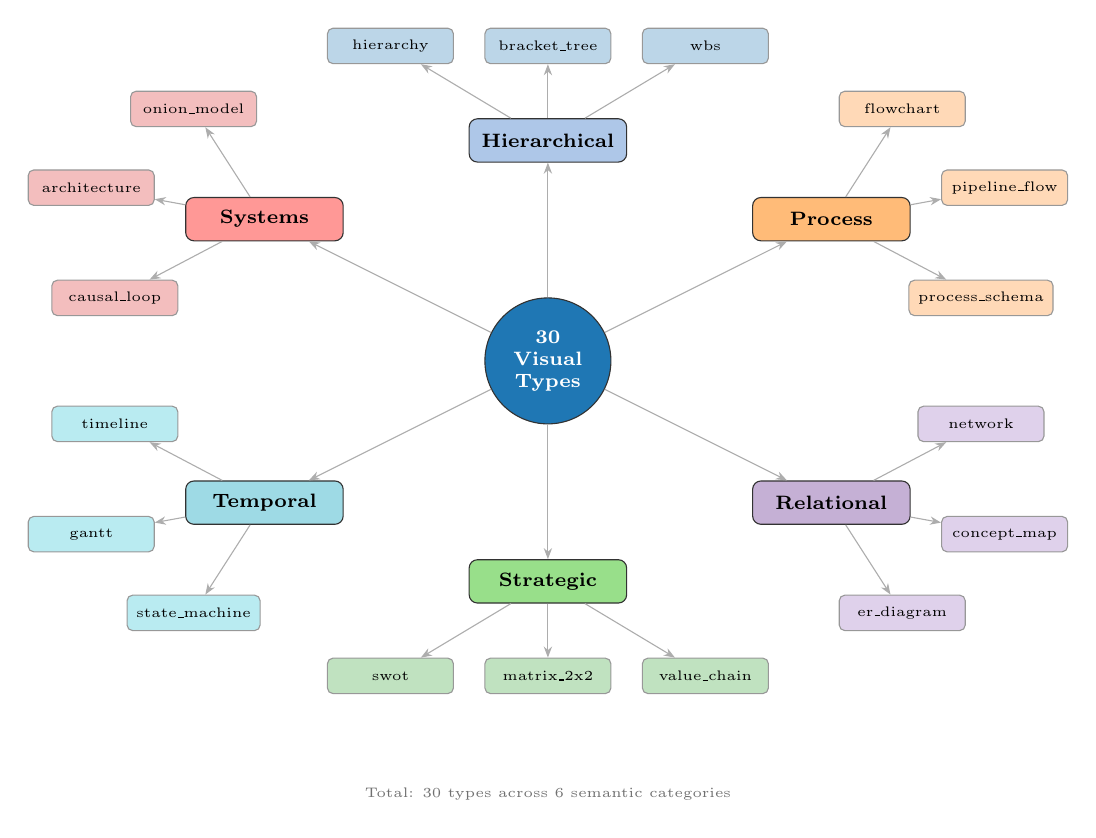
\begin{tikzpicture}[
  root/.style={draw=DG, circle, fill=CB, text=white,
               minimum size=1.6cm, font=\scriptsize\bfseries, align=center},
  cat/.style={draw=DG, rounded corners=3pt, fill=#1,
              minimum width=2.0cm, minimum height=0.55cm,
              font=\scriptsize\bfseries, align=center},
  leaf/.style={draw=DG!50, fill=#1!30, rounded corners=2pt,
               minimum width=1.6cm, minimum height=0.45cm,
               font=\tiny, align=center},
  earr/.style={draw=DG!40, thin, -{Stealth[length=4pt]}}
]
\node[root] (R) at (0,0) {30\\Visual\\Types};

% Category 1: Hierarchical (top)
\node[cat=LB]  (C1) at (0, 2.8)  {Hierarchical};
\draw[earr] (R)--(C1);
\node[leaf=CB] (L11) at (-2.0, 4.0) {hierarchy};
\node[leaf=CB] (L12) at (0,   4.0)  {bracket\_tree};
\node[leaf=CB] (L13) at (2.0, 4.0)  {wbs};
\foreach \n in {L11,L12,L13} \draw[earr] (C1)--(\n);

% Category 2: Flow (upper-right)
\node[cat=LO]  (C2) at (3.6, 1.8)  {Process};
\draw[earr] (R)--(C2);
\node[leaf=CO] (L21) at (4.5, 3.2) {flowchart};
\node[leaf=CO] (L22) at (5.8, 2.2) {pipeline\_flow};
\node[leaf=CO] (L23) at (5.5, 0.8) {process\_schema};
\foreach \n in {L21,L22,L23} \draw[earr] (C2)--(\n);

% Category 3: Relational (right)
\node[cat=LP]  (C3) at (3.6,-1.8)  {Relational};
\draw[earr] (R)--(C3);
\node[leaf=CP] (L31) at (5.5,-0.8) {network};
\node[leaf=CP] (L32) at (5.8,-2.2) {concept\_map};
\node[leaf=CP] (L33) at (4.5,-3.2) {er\_diagram};
\foreach \n in {L31,L32,L33} \draw[earr] (C3)--(\n);

% Category 4: Strategic (bottom)
\node[cat=LG]  (C4) at (0,-2.8)   {Strategic};
\draw[earr] (R)--(C4);
\node[leaf=CG] (L41) at (-2.0,-4.0){swot};
\node[leaf=CG] (L42) at (0,-4.0)   {matrix\_2x2};
\node[leaf=CG] (L43) at (2.0,-4.0) {value\_chain};
\foreach \n in {L41,L42,L43} \draw[earr] (C4)--(\n);

% Category 5: Temporal (lower-left)
\node[cat=LT]  (C5) at (-3.6,-1.8) {Temporal};
\draw[earr] (R)--(C5);
\node[leaf=CT] (L51) at (-5.5,-0.8){timeline};
\node[leaf=CT] (L52) at (-5.8,-2.2){gantt};
\node[leaf=CT] (L53) at (-4.5,-3.2){state\_machine};
\foreach \n in {L51,L52,L53} \draw[earr] (C5)--(\n);

% Category 6: Systems (left)
\node[cat=LR]  (C6) at (-3.6, 1.8) {Systems};
\draw[earr] (R)--(C6);
\node[leaf=CR] (L61) at (-5.5, 0.8){causal\_loop};
\node[leaf=CR] (L62) at (-5.8, 2.2){architecture};
\node[leaf=CR] (L63) at (-4.5, 3.2){onion\_model};
\foreach \n in {L61,L62,L63} \draw[earr] (C6)--(\n);

% Count badge
\node[font=\tiny, text=DG!70] at (0,-5.5)
  {Total: 30 types across 6 semantic categories};
\end{tikzpicture}
\caption{Taxonomy of 30 structural visual types supported by the TikZ blueprint
         system. Each type maps to a dedicated structural grammar prescribing
         layout, node styles, and required TikZ libraries.}
\label{fig:taxonomy}
\end{figure}

% ╔══════════════════════════════════════════════════════════════════════════╗
% ║  FIG 8 — Stage 5 LaTeX Compile-Repair Loop                              ║
% ╚══════════════════════════════════════════════════════════════════════════╝
\begin{figure}[h!]
\centering
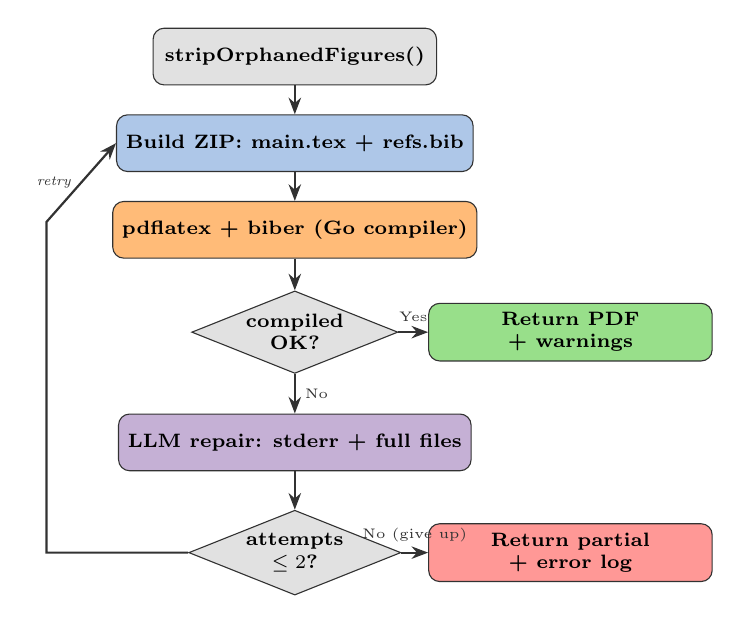
\begin{tikzpicture}[
  box/.style={draw=DG, rounded corners=4pt, fill=#1,
              minimum width=3.6cm, minimum height=0.72cm,
              align=center, font=\scriptsize\bfseries},
  dia/.style={draw=DG, diamond, aspect=2.5, fill=#1,
              align=center, font=\scriptsize\bfseries, inner sep=1pt},
  arr/.style={-{Stealth[length=6pt]}, thick, draw=DG},
  lbl/.style={font=\tiny, text=DG, midway}
]
\node[box=LGr] (strip)  at (0, 3.5) {stripOrphanedFigures()};
\node[box=LB]  (zip)    at (0, 2.4) {Build ZIP: main.tex + refs.bib};
\node[box=LO]  (comp)   at (0, 1.3) {pdflatex + biber (Go compiler)};
\node[dia=LGr] (ok)     at (0, 0.0) {compiled\\OK?};
\node[box=LG]  (done)   at (3.5, 0.0){Return PDF\\+ warnings};
\node[box=LP]  (repair) at (0,-1.4) {LLM repair: stderr + full files};
\node[dia=LGr] (att)    at (0,-2.8) {attempts\\$\leq 2$?};
\node[box=LR]  (fail)   at (3.5,-2.8){Return partial\\+ error log};

\draw[arr] (strip)--(zip);
\draw[arr] (zip)--(comp);
\draw[arr] (comp)--(ok);
\draw[arr] (ok)--node[lbl, above]{Yes}(done);
\draw[arr] (ok)--node[lbl, right]{No}(repair);
\draw[arr] (repair)--(att);
\draw[arr] (att)--node[lbl, above]{No (give up)}(fail);
\draw[arr] (att.west)--++(-1.8,0)--++(0,4.2)--(zip.west)
  node[pos=0.5, left, font=\tiny\itshape, text=DG]{retry};
\end{tikzpicture}
\caption{Stage\,5 compile-validate-repair loop. Orphaned \texttt{\textbackslash{}includegraphics}
         commands are stripped as a heuristic pre-repair step; up to two LLM-driven
         repair iterations follow compiler failure.}
\label{fig:stage5}
\end{figure}

% ╔══════════════════════════════════════════════════════════════════════════╗
% ║  FIG 9 — Real-Data Guard State Machine                                  ║
% ╚══════════════════════════════════════════════════════════════════════════╝
\begin{figure}[h!]
\centering
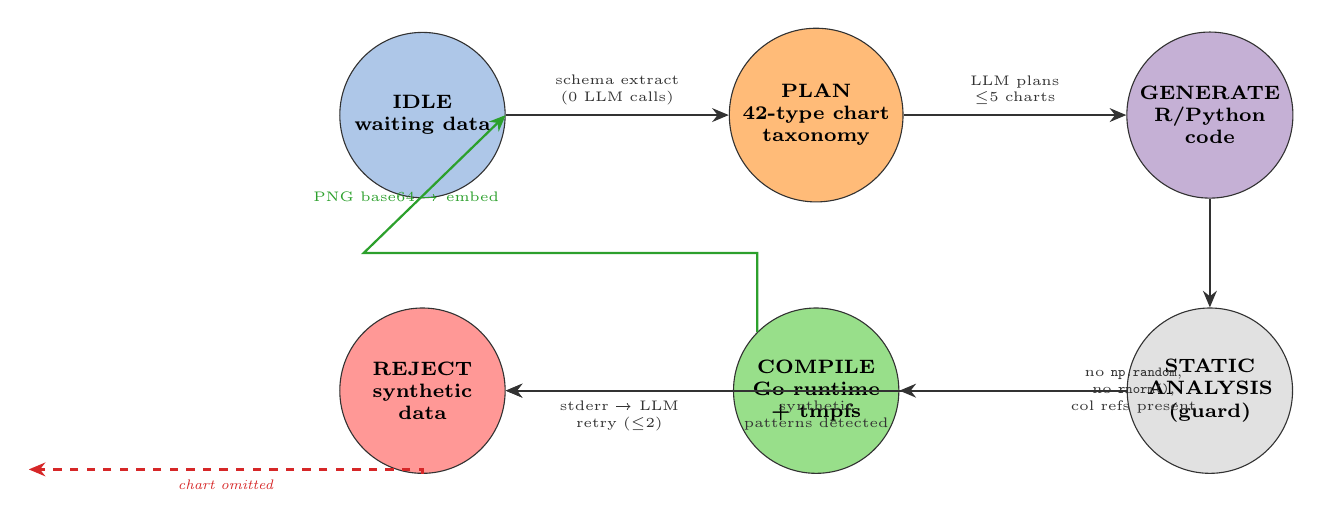
\begin{tikzpicture}[
  st/.style={draw=DG, circle, fill=#1, minimum size=2.1cm,
             align=center, font=\scriptsize\bfseries, inner sep=2pt},
  arr/.style={-{Stealth[length=6pt,width=5pt]}, thick, draw=DG},
  lbl/.style={font=\tiny, text=DG, align=center, text width=2.6cm}
]
\node[st=LB]   (s0) at (0,0)     {IDLE\\waiting data};
\node[st=LO]   (s1) at (5.0,0)   {PLAN\\42-type chart\\taxonomy};
\node[st=LP]   (s2) at (10,0)    {GENERATE\\R/Python\\code};
\node[st=LGr]  (s3) at (10,-3.5) {STATIC\\ANALYSIS\\(guard)};
\node[st=LG]   (s4) at (5.0,-3.5){COMPILE\\Go runtime\\+ tmpfs};
\node[st=LR]   (s5) at (0,-3.5)  {REJECT\\synthetic\\data};

\draw[arr] (s0)--node[above,lbl]{schema extract\\(0 LLM calls)}(s1);
\draw[arr] (s1)--node[above,lbl]{LLM plans\\$\leq$5 charts}(s2);
\draw[arr] (s2)--(s3);
\draw[arr] (s3)--node[right,lbl,text width=2.8cm]{no \texttt{np.random},\\no \texttt{rnorm()},\\col refs present}(s4);
\draw[arr] (s3)--node[below,lbl]{synthetic\\patterns detected}(s5);
\draw[arr] (s4)--node[below,lbl]{stderr → LLM\\retry ($\leq$2)}(s5);
\draw[arr, CG] (s4.north west)--++(0,1.0)--++(-5.0,0)--(s0.east)
  node[pos=0.3, above, font=\tiny, text=CG]{PNG base64 → embed};
\draw[arr, CR, dashed] (s5)--++(0,-1.0)--++(-5,0)
  node[pos=0.5, below, font=\tiny\itshape, text=CR]{chart omitted};
\end{tikzpicture}
\caption{Real-data guard state machine for the analytics pipeline. A static
         analysis pass detects synthetic data patterns (\texttt{np.random.*},
         \texttt{rnorm()}, \texttt{runif()}) before compiler invocation,
         preventing hallucinated charts.}
\label{fig:data-guard}
\end{figure}

% ╔══════════════════════════════════════════════════════════════════════════╗
% ║  FIG 10 — LCS Figure-Label Reconciliation                               ║
% ╚══════════════════════════════════════════════════════════════════════════╝
\begin{figure}[h!]
\centering
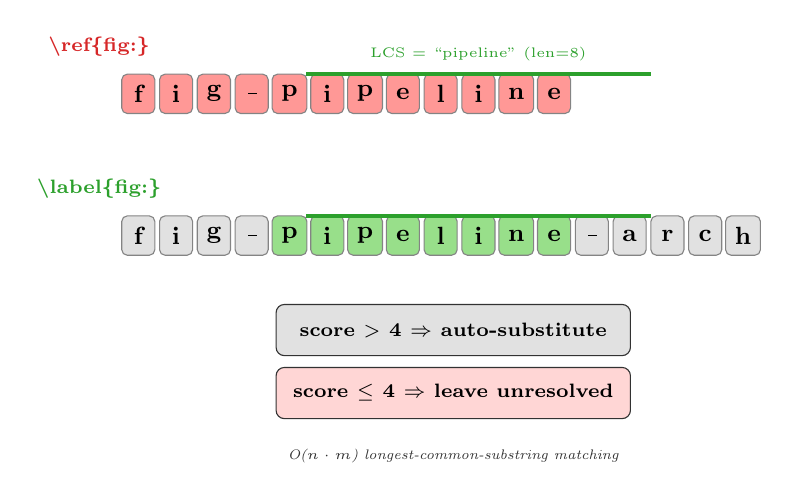
\begin{tikzpicture}[
  sbox/.style={draw=DG!60, fill=#1, rounded corners=2pt,
               minimum width=0.42cm, minimum height=0.5cm,
               font=\small\bfseries, align=center},
  lbox/.style={draw=DG, fill=#1, rounded corners=3pt,
               minimum width=4.5cm, minimum height=0.65cm,
               align=center, font=\scriptsize\bfseries},
  arr/.style={-{Stealth[length=5pt]}, thick, draw=DG}
]
% ref string
\node[font=\scriptsize\bfseries, text=CR] at (-0.5, 1.6) {\textbackslash ref\{fig:\}};
\foreach \i/\c/\ch in {
  0/LR/f, 1/LR/i, 2/LR/g, 3/LR/\_, 4/LR/p, 5/LR/i, 6/LR/p,
  7/LR/e, 8/LR/l, 9/LR/i, 10/LR/n, 11/LR/e} {
  \node[sbox=\c] at (\i*0.48, 1.0) {\ch};
}

% label string
\node[font=\scriptsize\bfseries, text=CG] at (-0.5, -0.2) {\textbackslash label\{fig:\}};
\foreach \i/\c/\ch in {
  0/LGr/f, 1/LGr/i, 2/LGr/g, 3/LGr/\_, 4/LG/p, 5/LG/i, 6/LG/p,
  7/LG/e, 8/LG/l, 9/LG/i, 10/LG/n, 11/LG/e, 12/LGr/\_, 13/LGr/a, 14/LGr/r, 15/LGr/c, 16/LGr/h} {
  \node[sbox=\c] at (\i*0.48, -0.8) {\ch};
}

% LCS underline
\draw[very thick, CG] (1.92+0.21, 1.25)--(6.72-0.21,1.25);
\draw[very thick, CG] (1.92+0.21,-0.55)--(6.72-0.21,-0.55);
\node[font=\tiny, text=CG] at (4.32, 1.5) {LCS = ``pipeline'' (len=8)};

% Threshold
\node[lbox=LGr] at (4.0, -2.0) {score $>$ 4 $\Rightarrow$ auto-substitute};
\node[lbox=LR!40] at (4.0,-2.8) {score $\leq$ 4 $\Rightarrow$ leave unresolved};

\node[font=\tiny\itshape, text=DG, align=center] at (4.0,-3.6)
  {O($n \cdot m$) longest-common-substring matching};
\end{tikzpicture}
\caption{LCS-based figure-label reconciliation. When \texttt{\textbackslash ref\{fig:X\}} does not
         match any defined \texttt{\textbackslash label\{fig:Y\}}, the longest common substring
         determines the best match candidate; a threshold of $>4$ characters
         prevents spurious substitutions.}
\label{fig:lcs}
\end{figure}

% ╔══════════════════════════════════════════════════════════════════════════╗
% ║  FIG 11 — Multilanguage Preamble Decision Tree                          ║
% ╚══════════════════════════════════════════════════════════════════════════╝
\begin{figure}[h!]
\centering
\begin{tikzpicture}[
  dia/.style={draw=DG, diamond, aspect=2.4, fill=LGr,
              align=center, font=\scriptsize\bfseries, inner sep=1pt},
  leaf/.style={draw=DG, rounded corners=3pt, fill=#1,
               minimum width=3.0cm, minimum height=0.8cm,
               align=center, font=\scriptsize\bfseries, text width=2.8cm},
  arr/.style={-{Stealth[length=5pt]}, thick, draw=DG},
  y/.style={font=\tiny, text=CG, midway},
  n/.style={font=\tiny, text=CR, midway}
]
\node[dia] (q1) at (0, 0)   {lang\\= kk?};
\node[dia] (q2) at (0,-2.0) {CYRILLIC\\lang?};
\node[dia] (q3) at (0,-4.0) {lang\\$\neq$ en?};

\node[leaf=LT] (kk) at (5.0, 0.0)
  {XeLaTeX + fontspec\\Inter font\\{[kazakh]}\{babel\}};
\node[leaf=LP] (cy) at (5.0,-2.0)
  {T2A + utf8\\{[russian,english]}\{babel\}\\25 lang map};
\node[leaf=LO] (lt) at (5.0,-4.0)
  {T1 + utf8\\{[lang,english]}\{babel\}};
\node[leaf=LGr] (en) at (5.0,-6.0)
  {T1 + utf8\\(no babel)};

\node[dia] (q4) at (0,-6.0) {lang\\= en?};

\draw[arr] (q1)--node[y,above]{Yes}(kk);
\draw[arr] (q1)--node[n,right]{No}(q2);
\draw[arr] (q2)--node[y,above]{Yes}(cy);
\draw[arr] (q2)--node[n,right]{No}(q3);
\draw[arr] (q3)--node[y,above]{Yes}(lt);
\draw[arr] (q3)--node[n,right]{No}(q4);
\draw[arr] (q4)--node[y,above]{Yes}(en);

\node[font=\tiny\itshape, text=DG] at (0,-7.2)
  {BABEL\_LANG\_MAP covers 25 languages};
\end{tikzpicture}
\caption{Four-branch deterministic multilanguage preamble synthesizer.
         Encoding stacks are selected based on writing system:
         Kazakh (XeLaTeX), Cyrillic scripts (T2A/pdflatex),
         other Latin scripts (T1/babel), and English (T1 only).}
\label{fig:preamble}
\end{figure}

% ╔══════════════════════════════════════════════════════════════════════════╗
% ║  FIG 12 — Multimodal Context Assembly per Section                       ║
% ╚══════════════════════════════════════════════════════════════════════════╝
\begin{figure}[h!]
\centering
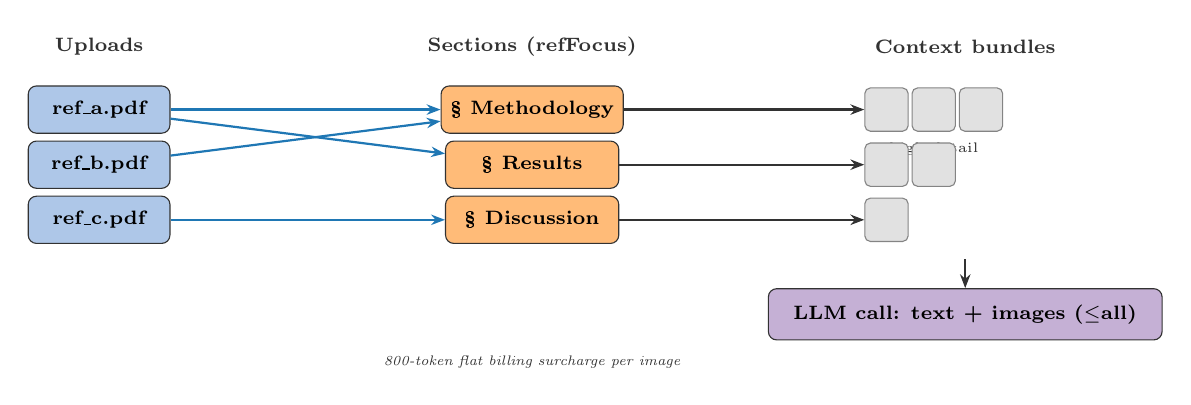
\begin{tikzpicture}[
  pdf/.style={draw=DG, fill=LB, rounded corners=3pt,
              minimum width=1.8cm, minimum height=0.6cm,
              font=\scriptsize\bfseries, align=center},
  sec/.style={draw=DG, fill=LO, rounded corners=3pt,
              minimum width=2.2cm, minimum height=0.6cm,
              font=\scriptsize\bfseries, align=center},
  img/.style={draw=DG!60, fill=LGr, rounded corners=2pt,
              minimum width=0.55cm, minimum height=0.55cm,
              font=\tiny, align=center},
  ctx/.style={draw=DG, fill=LP, rounded corners=3pt,
              minimum width=5cm, minimum height=0.65cm,
              font=\scriptsize\bfseries, align=center},
  arr/.style={-{Stealth[length=5pt]}, thick, draw=DG}
]
% PDFs
\node[font=\scriptsize\bfseries, text=DG] at (-5.5, 2.2) {Uploads};
\node[pdf] (p1) at (-5.5, 1.4) {ref\_a.pdf};
\node[pdf] (p2) at (-5.5, 0.7) {ref\_b.pdf};
\node[pdf] (p3) at (-5.5, 0.0) {ref\_c.pdf};

% Section planning (refFocus)
\node[font=\scriptsize\bfseries, text=DG] at (0, 2.2) {Sections (refFocus)};
\node[sec] (s1) at (0, 1.4) {§ Methodology};
\node[sec] (s2) at (0, 0.7) {§ Results};
\node[sec] (s3) at (0, 0.0) {§ Discussion};

% Mapping arrows
\draw[arr, CB] (p1)--(s1); \draw[arr, CB] (p1)--(s2);
\draw[arr, CB] (p2)--(s1); \draw[arr, CB] (p3)--(s3);

% Images from PDFs
\node[font=\scriptsize\bfseries, text=DG] at (5.5, 2.2) {Context bundles};
\node[img] (i1) at (4.5, 1.4) {\(\square\)};
\node[img] at (5.1, 1.4) {\(\square\)};
\node[img] at (5.7, 1.4) {\(\square\)};
\node[font=\tiny, text=DG] at (5.1, 0.9) {high detail};
\draw[arr] (s1)--(i1);

\node[img] (i2) at (4.5, 0.7) {\(\square\)};
\node[img] at (5.1, 0.7) {\(\square\)};
\draw[arr] (s2)--(i2);

\node[img] (i3) at (4.5, 0.0) {\(\square\)};
\draw[arr] (s3)--(i3);

% Final LLM call
\node[ctx] (llm) at (5.5, -1.2) {LLM call: text + images ($\leq$all)};
\draw[arr] (5.5, -0.5)--(llm);

\node[font=\tiny\itshape, text=DG, align=center] at (0,-1.8)
  {800-token flat billing surcharge per image};
\end{tikzpicture}
\caption{Section-scoped multimodal context assembly. Each section receives
         only images from its \texttt{refFocus} uploads at \texttt{detail=high},
         enabling targeted visual grounding with deterministic billing correction.}
\label{fig:multimodal}
\end{figure}

% ╔══════════════════════════════════════════════════════════════════════════╗
% ║  FIG 13 — JWT Double-Validation Authentication                          ║
% ╚══════════════════════════════════════════════════════════════════════════╝
\begin{figure}[h!]
\centering
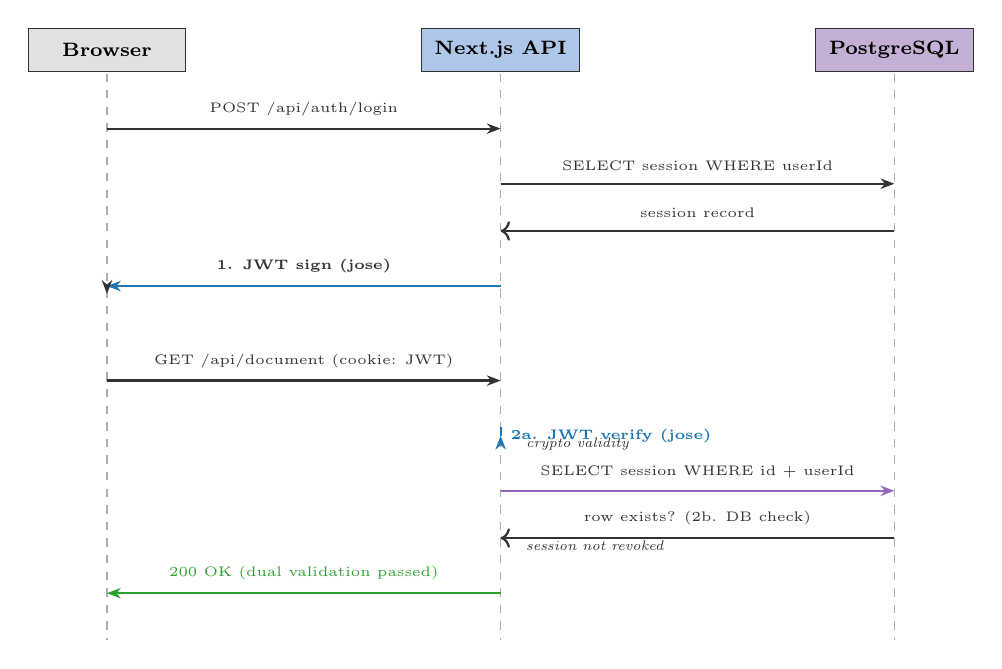
\begin{tikzpicture}[
  actor/.style={draw=DG, fill=#1, minimum width=2.0cm, minimum height=0.55cm,
                align=center, font=\scriptsize\bfseries},
  line/.style={draw=DG!40, dashed, thin},
  msg/.style={-{Stealth[length=5pt]}, thick, draw=#1},
  note/.style={font=\tiny, text=DG, midway, above=1pt}
]
% Actors
\node[actor=LGr] (client) at (0,0)   {Browser};
\node[actor=LB]  (server) at (5,0)   {Next.js API};
\node[actor=LP]  (db)     at (10,0)  {PostgreSQL};

% Lifelines
\draw[line] (0,-0.3)--(0,-7.5);
\draw[line] (5,-0.3)--(5,-7.5);
\draw[line] (10,-0.3)--(10,-7.5);

% Messages
\draw[msg=DG] (0,-1.0)--node[note]{POST /api/auth/login}(5,-1.0);
\draw[msg=DG] (5,-1.7)--node[note]{SELECT session WHERE userId}(10,-1.7);
\draw[msg=DG,<-] (5,-2.3)--node[note]{session record}(10,-2.3);
\draw[msg=CB] (5,-3.0)--node[note,above=1pt]{\textbf{1. JWT sign (jose)}}(0,-3.0);
\draw[msg=DG] (0,-3.0)--++(0,-0.1);  % recv tick

% Second request
\draw[msg=DG] (0,-4.2)--node[note]{GET /api/document (cookie: JWT)}(5,-4.2);
\draw[msg=CB] (5,-4.9)--++(0,0) node[right, font=\tiny, text=CB]
  {\textbf{2a. JWT verify (jose)}};
\draw[msg=CP] (5,-5.6)--node[note]{SELECT session WHERE id + userId}(10,-5.6);
\draw[msg=DG,<-] (5,-6.2)--node[note]{row exists? (2b. DB check)}(10,-6.2);
\draw[msg=CG] (5,-6.9)--node[note, text=CG]{200 OK (dual validation passed)}(0,-6.9);

% Labels
\node[font=\tiny\itshape, text=DG, anchor=west] at (5.2,-5.0)
  {crypto validity};
\node[font=\tiny\itshape, text=DG, anchor=west] at (5.2,-6.3)
  {session not revoked};
\end{tikzpicture}
\caption{JWT double-validation authentication flow. Every request validates
         JWT cryptographic integrity \emph{and} performs a database session
         lookup, enabling immediate server-side session revocation.}
\label{fig:jwt}
\end{figure}

% ╔══════════════════════════════════════════════════════════════════════════╗
% ║  FIG 14 — Token-to-Character Billing System                             ║
% ╚══════════════════════════════════════════════════════════════════════════╝
\begin{figure}[h!]
\centering
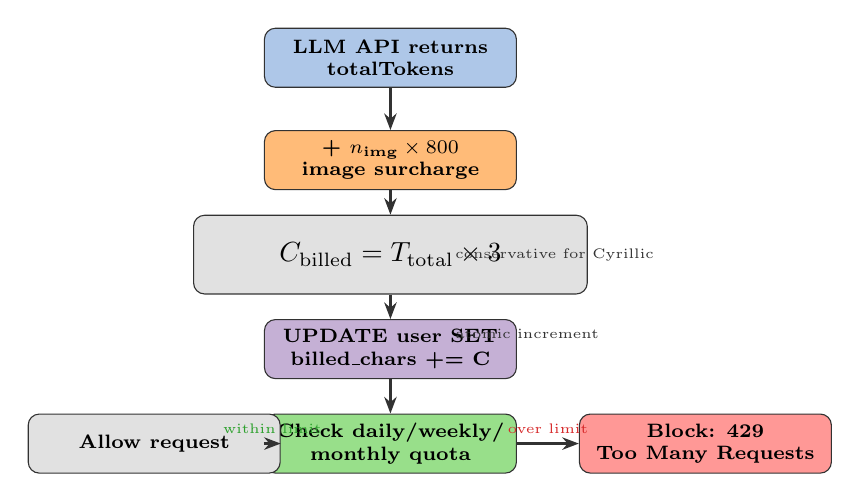
\begin{tikzpicture}[
  box/.style={draw=DG, rounded corners=4pt, fill=#1,
              minimum width=3.2cm, minimum height=0.75cm,
              align=center, font=\scriptsize\bfseries},
  fml/.style={draw=DG, rounded corners=4pt, fill=LGr,
              minimum width=5cm, minimum height=1.0cm,
              align=center, font=\normalsize},
  arr/.style={-{Stealth[length=6pt]}, thick, draw=DG},
  note/.style={font=\tiny, text=DG, anchor=west}
]
\node[box=LB]  (tok)   at (0, 2.5) {LLM API returns\\totalTokens};
\node[box=LO]  (img)   at (0, 1.2) {+ $n_{\text{img}} \times 800$\\image surcharge};
\node[fml]     (fml)   at (0, 0.0) {$C_{\text{billed}} = T_{\text{total}} \times 3$};
\node[box=LP]  (db)    at (0,-1.2) {UPDATE user SET\\billed\_chars += C};
\node[box=LG]  (quota) at (0,-2.4) {Check daily/weekly/\\monthly quota};
\node[box=LR]  (block) at (4.0,-2.4){Block: 429\\Too Many Requests};
\node[box=LGr] (ok)    at (-3.0,-2.4){Allow request};

\draw[arr] (tok)--(img);
\draw[arr] (img)--(fml);
\draw[arr] (fml)--(db);
\draw[arr] (db)--(quota);
\draw[arr] (quota)--node[above,font=\tiny,text=CR]{over limit}(block);
\draw[arr] (quota)--node[above,font=\tiny,text=CG]{within limit}(ok);

\node[note] at (0.7, 0.0) {conservative for Cyrillic};
\node[note] at (0.7,-1.0) {atomic increment};
\end{tikzpicture}
\caption{Token-to-character billing pipeline. A deterministic \(\times 3\)
         multiplier converts LLM-reported tokens to billed characters, with
         a flat 800-token surcharge per vision image.}
\label{fig:billing}
\end{figure}

% ╔══════════════════════════════════════════════════════════════════════════╗
% ║  FIG 15 — Docker 9-Service Topology                                     ║
% ╚══════════════════════════════════════════════════════════════════════════╝
\begin{figure}[h!]
\centering
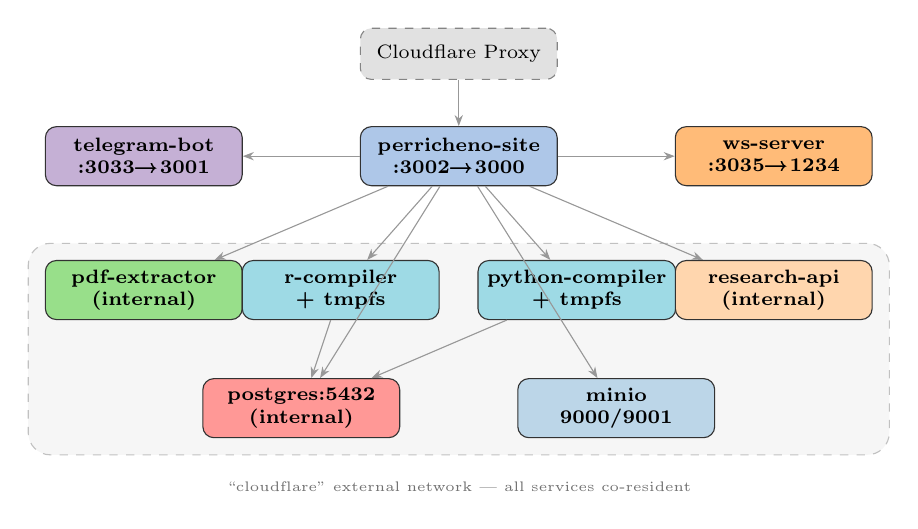
\begin{tikzpicture}[
  svc/.style={draw=DG, rounded corners=4pt, fill=#1,
              minimum width=2.5cm, minimum height=0.75cm,
              align=center, font=\scriptsize\bfseries},
  pub/.style={draw=DG!60, dashed, fill=#1, rounded corners=4pt,
              minimum width=2.5cm, minimum height=0.65cm,
              align=center, font=\scriptsize},
  conn/.style={draw=DG!50, thin, -{Stealth[length=4pt]}},
  note/.style={font=\tiny, text=DG!70}
]
% Public-facing
\node[pub=LGr] (cf) at (0, 4.5) {Cloudflare Proxy};
\node[svc=LB]  (web) at (0, 3.2) {perricheno-site\\:3002→3000};
\node[svc=LO]  (ws)  at (4.0, 3.2) {ws-server\\:3035→1234};
\node[svc=LP]  (bot) at (-4.0, 3.2){telegram-bot\\:3033→3001};

% Internal compute
\node[svc=LG]  (pdf) at (-4.0, 1.5){pdf-extractor\\(internal)};
\node[svc=LT]  (rco) at (-1.5, 1.5){r-compiler\\+ tmpfs};
\node[svc=LT]  (pyc) at (1.5, 1.5) {python-compiler\\+ tmpfs};
\node[svc=LO!60](res) at (4.0, 1.5) {research-api\\(internal)};

% Data
\node[svc=LR]  (pg) at (-2.0, 0.0){postgres:5432\\(internal)};
\node[svc=CB!30](minio) at (2.0, 0.0){minio\\9000/9001};

% Connections
\draw[conn] (cf)--(web);
\draw[conn] (web)--(ws);
\draw[conn] (web)--(pdf);
\draw[conn] (web)--(rco);
\draw[conn] (web)--(pyc);
\draw[conn] (web)--(res);
\draw[conn] (web)--(bot);
\draw[conn] (web)--(pg);
\draw[conn] (web)--(minio);
\draw[conn] (rco)--(pg);
\draw[conn] (pyc)--(pg);

% Network boundary
\begin{scope}[on background layer]
  \node[draw=DG!30, dashed, rounded corners=8pt, fit=(pdf)(rco)(pyc)(res)(pg)(minio),
        inner sep=6pt, fill=LGr!30] {};
\end{scope}
\node[note] at (0,-1.0) {``cloudflare'' external network — all services co-resident};
\end{tikzpicture}
\caption{Docker Compose nine-service topology. Internal services have no published
         ports; \texttt{r-compiler} and \texttt{python-compiler} mount ephemeral
         \texttt{tmpfs} volumes for zero-persistence code execution.}
\label{fig:docker}
\end{figure}

% ╔══════════════════════════════════════════════════════════════════════════╗
% ║  FIG 16 — Bi-Modal API Dispatch                                         ║
% ╚══════════════════════════════════════════════════════════════════════════╝
\begin{figure}[h!]
\centering
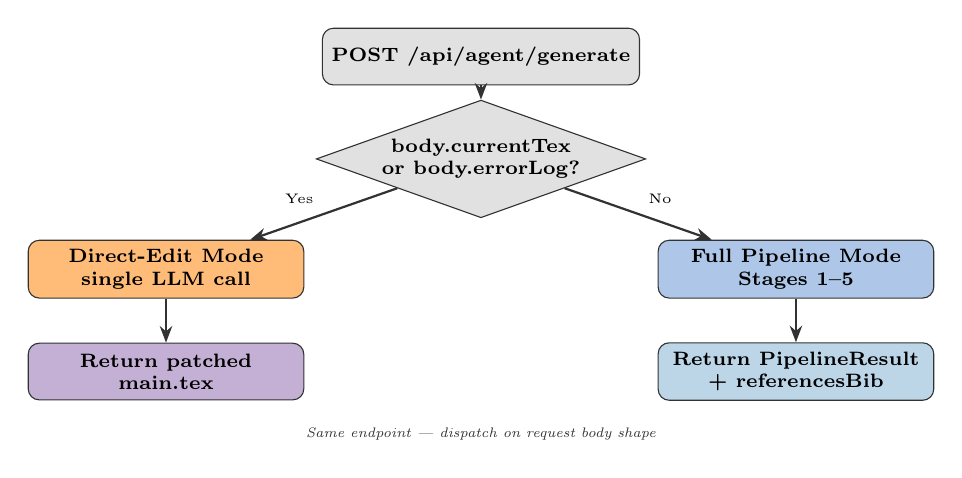
\begin{tikzpicture}[
  box/.style={draw=DG, rounded corners=4pt, fill=#1,
              minimum width=3.5cm, minimum height=0.72cm,
              align=center, font=\scriptsize\bfseries},
  dia/.style={draw=DG, diamond, aspect=2.8, fill=LGr,
              align=center, font=\scriptsize\bfseries, inner sep=1pt},
  arr/.style={-{Stealth[length=6pt]}, thick, draw=DG}
]
\node[box=LGr]  (req)  at (0, 3.0)  {POST /api/agent/generate};
\node[dia]      (gate) at (0, 1.7)  {body.currentTex\\or body.errorLog?};
\node[box=LO]   (edit) at (-4.0, 0.3){Direct-Edit Mode\\single LLM call};
\node[box=LB]   (pipe) at (4.0, 0.3) {Full Pipeline Mode\\Stages 1--5};
\node[box=LP]   (ea)   at (-4.0,-1.0){Return patched\\main.tex};
\node[box=CB!30](pa)   at (4.0,-1.0) {Return PipelineResult\\+ referencesBib};

\draw[arr] (req)--(gate);
\draw[arr] (gate)--node[above left, font=\tiny]{Yes}(edit);
\draw[arr] (gate)--node[above right, font=\tiny]{No}(pipe);
\draw[arr] (edit)--(ea);
\draw[arr] (pipe)--(pa);

\node[font=\tiny\itshape, text=DG, align=center] at (0,-1.8)
  {Same endpoint — dispatch on request body shape};
\end{tikzpicture}
\caption{Bi-modal API dispatch. A single endpoint serves both full
         six-stage document generation and lightweight single-call
         direct editing, branching on the presence of existing document state.}
\label{fig:bimodal}
\end{figure}

% ╔══════════════════════════════════════════════════════════════════════════╗
% ║  FIG 17 — CrossRef DOI Enrichment Pipeline                              ║
% ╚══════════════════════════════════════════════════════════════════════════╝
\begin{figure}[h!]
\centering
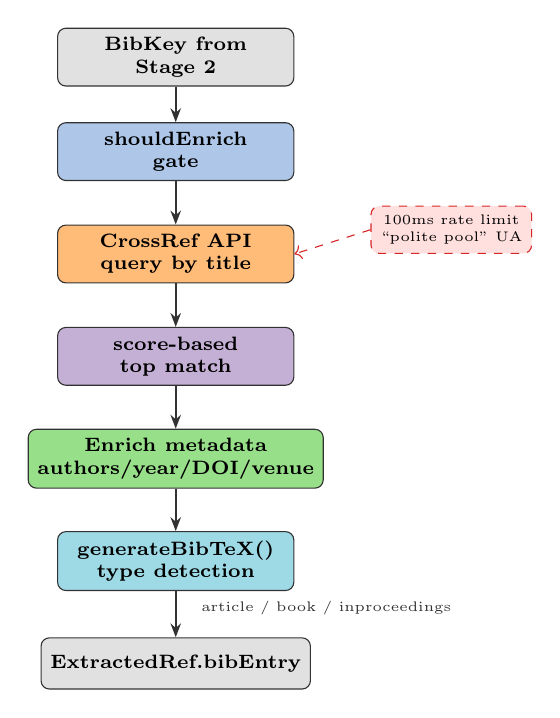
\begin{tikzpicture}[
  box/.style={draw=DG, rounded corners=3pt, fill=#1,
              minimum width=3.0cm, minimum height=0.65cm,
              align=center, font=\scriptsize\bfseries},
  arr/.style={-{Stealth[length=5pt]}, thick, draw=DG},
  rate/.style={draw=CR, dashed, rounded corners=3pt, fill=LR!30,
               minimum width=2.0cm, minimum height=0.55cm,
               align=center, font=\tiny, anchor=south}
]
% Pipeline
\node[box=LGr] (bibkey)  at (0, 0)    {BibKey from\\Stage 2};
\node[box=LB]  (gate)    at (0,-1.2)  {shouldEnrich\\gate};
\node[box=LO]  (search)  at (0,-2.5)  {CrossRef API\\query by title};
\node[box=LP]  (match)   at (0,-3.8)  {score-based\\top match};
\node[box=LG]  (enrich)  at (0,-5.1)  {Enrich metadata\\authors/year/DOI/venue};
\node[box=LT]  (bibtex)  at (0,-6.4)  {generateBibTeX()\\type detection};
\node[box=LGr] (out)     at (0,-7.7)  {ExtractedRef.bibEntry};

\draw[arr] (bibkey)--(gate);
\draw[arr] (gate)--(search);
\draw[arr] (search)--(match);
\draw[arr] (match)--(enrich);
\draw[arr] (enrich)--(bibtex);
\draw[arr] (bibtex)--(out);

% Rate limiter
\node[rate] (rl) at (3.5,-2.5) {100ms rate limit\\``polite pool'' UA};
\draw[draw=CR, dashed, ->, thin] (rl.west)--(search.east);

% BibTeX types
\node[font=\tiny, text=DG, align=left, anchor=west] at (0.2,-7.0)
  {article / book / inproceedings};
\end{tikzpicture}
\caption{CrossRef DOI enrichment pipeline (Stage\,2.7). A polite-pool
         User-Agent and 100\,ms inter-request delay comply with CrossRef
         API guidelines; entry type is inferred from metadata fields.}
\label{fig:crossref}
\end{figure}

% ╔══════════════════════════════════════════════════════════════════════════╗
% ║  FIG 18 — Telegram QR Auth Polling Flow                                 ║
% ╚══════════════════════════════════════════════════════════════════════════╝
\begin{figure}[h!]
\centering
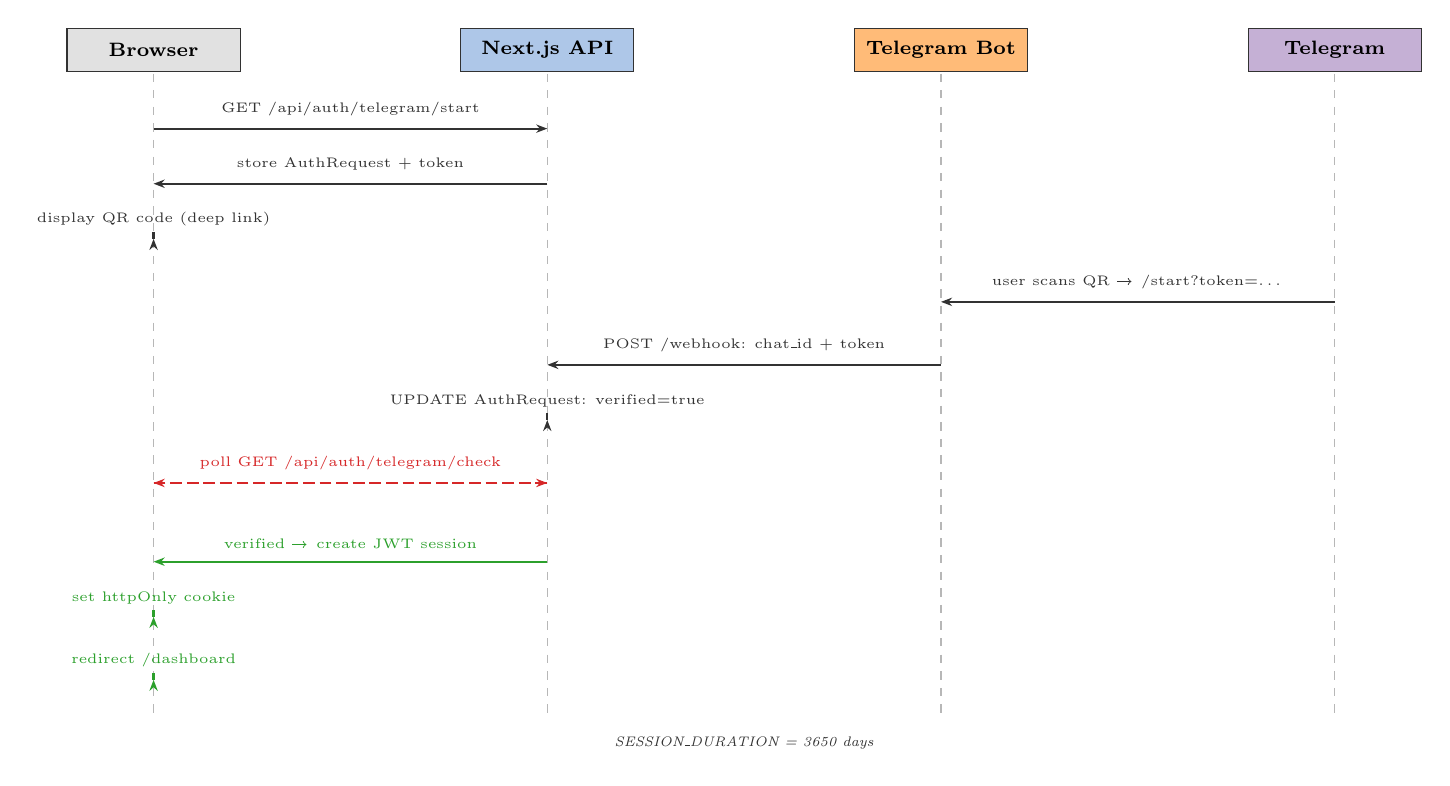
\begin{tikzpicture}[
  actor/.style={draw=DG, fill=#1, minimum width=2.2cm, minimum height=0.55cm,
                align=center, font=\scriptsize\bfseries},
  msg/.style={-{Stealth[length=4pt]}, draw=DG, thick},
  note/.style={font=\tiny, text=DG, midway, above=1pt},
  dline/.style={draw=DG!35, dashed, thin}
]
\node[actor=LGr] (ui)  at (0,0)   {Browser};
\node[actor=LB]  (api) at (5,0)   {Next.js API};
\node[actor=LO]  (bot) at (10,0)  {Telegram Bot};
\node[actor=LP]  (tg)  at (15,0)  {Telegram};

\draw[dline] (0,-0.3)--(0,-8.5);
\draw[dline] (5,-0.3)--(5,-8.5);
\draw[dline] (10,-0.3)--(10,-8.5);
\draw[dline] (15,-0.3)--(15,-8.5);

\draw[msg] (0,-1.0)--node[note]{GET /api/auth/telegram/start}(5,-1.0);
\draw[msg] (5,-1.7)--node[note]{store AuthRequest + token}(0,-1.7);
\draw[msg] (0,-2.4)--node[note]{display QR code (deep link)}(0,-2.4);

\draw[msg] (15,-3.2)--node[note]{user scans QR → /start?token=…}(10,-3.2);
\draw[msg] (10,-4.0)--node[note]{POST /webhook: chat\_id + token}(5,-4.0);
\draw[msg] (5,-4.7)--node[note]{UPDATE AuthRequest: verified=true}(5,-4.7);

\draw[msg, draw=CR, dashed] (0,-5.5)--node[note, text=CR]{poll GET /api/auth/telegram/check}(5,-5.5);
\draw[msg, draw=CR, dashed] (5,-5.5)--(0,-5.5);

\draw[msg, draw=CG] (5,-6.5)--node[note, text=CG]{verified → create JWT session}(0,-6.5);
\draw[msg, draw=CG] (0,-7.2)--node[note, text=CG]{set httpOnly cookie}(0,-7.2);
\draw[msg, CG] (0,-8.0)--node[note, text=CG]{redirect /dashboard}(0,-8.0);

\node[font=\tiny\itshape, text=DG] at (7.5,-8.8)
  {SESSION\_DURATION = 3650 days};
\end{tikzpicture}
\caption{Telegram QR deep-link authentication flow. Browser polls until
         the bot webhook signals token verification; a JWT session
         is then issued with a 10-year duration.}
\label{fig:telegram}
\end{figure}

% ╔══════════════════════════════════════════════════════════════════════════╗
% ║  FIG 19 — Reference Quality Tier Pyramid                                ║
% ╚══════════════════════════════════════════════════════════════════════════╝
\begin{figure}[h!]
\centering
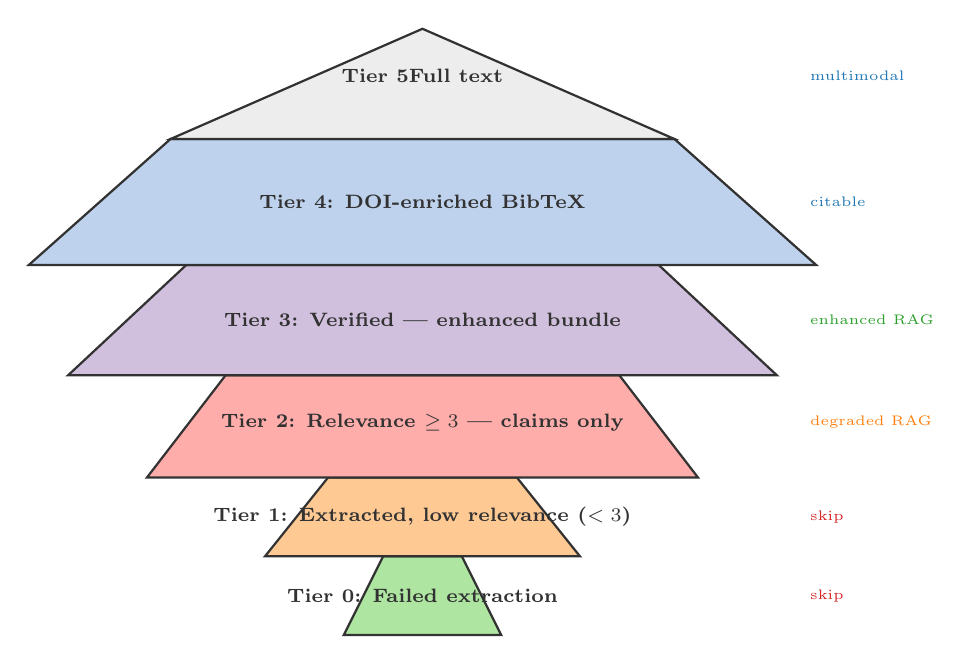
\begin{tikzpicture}
% Pyramid via filled polygons
\fill[LG!80, draw=DG, thick]
  (-1.0,-2.5) -- (1.0,-2.5) -- (0.5,-1.5) -- (-0.5,-1.5) -- cycle;
\fill[LO!80, draw=DG, thick]
  (-2.0,-1.5) -- (2.0,-1.5) -- (1.2,-0.5) -- (-1.2,-0.5) -- cycle;
\fill[LR!80, draw=DG, thick]
  (-3.5,-0.5) -- (3.5,-0.5) -- (2.5, 0.8) -- (-2.5, 0.8) -- cycle;
\fill[LP!80, draw=DG, thick]
  (-4.5, 0.8) -- (4.5, 0.8) -- (3.0, 2.2) -- (-3.0, 2.2) -- cycle;
\fill[LB!80, draw=DG, thick]
  (-5.0, 2.2) -- (5.0, 2.2) -- (3.2, 3.8) -- (-3.2, 3.8) -- cycle;
\fill[LGr!60, draw=DG, thick]
  (-3.2, 3.8) -- (3.2, 3.8) -- (0, 5.2) -- cycle;

% Labels inside
\node[font=\scriptsize\bfseries, text=DG] at (0,-2.0) {Tier 0: Failed extraction};
\node[font=\scriptsize\bfseries, text=DG] at (0,-1.0) {Tier 1: Extracted, low relevance ($<3$)};
\node[font=\scriptsize\bfseries, text=DG] at (0, 0.2) {Tier 2: Relevance $\geq 3$ — claims only};
\node[font=\scriptsize\bfseries, text=DG] at (0, 1.5) {Tier 3: Verified — enhanced bundle};
\node[font=\scriptsize\bfseries, text=DG] at (0, 3.0) {Tier 4: DOI-enriched BibTeX};
\node[font=\scriptsize\bfseries, text=DG] at (0, 4.6) {Tier 5\\Full text};

% Side annotations
\node[font=\tiny, text=CR, anchor=west] at (4.8,-2.0) {skip};
\node[font=\tiny, text=CR, anchor=west] at (4.8,-1.0) {skip};
\node[font=\tiny, text=CO, anchor=west] at (4.8, 0.2) {degraded RAG};
\node[font=\tiny, text=CG, anchor=west] at (4.8, 1.5) {enhanced RAG};
\node[font=\tiny, text=CB, anchor=west] at (4.8, 3.0) {citable};
\node[font=\tiny, text=CB, anchor=west] at (4.8, 4.6) {multimodal};
\end{tikzpicture}
\caption{Reference quality tier pyramid. Extraction failure and low relevance
         ($<3/10$) exclude a source; verified high-relevance documents receive
         full-text enhanced bundles for Stage\,3 drafting.}
\label{fig:pyramid}
\end{figure}

% ╔══════════════════════════════════════════════════════════════════════════╗
% ║  FIG 20 — Stage 1 Planning + Fallback                                   ║
% ╚══════════════════════════════════════════════════════════════════════════╝
\begin{figure}[h!]
\centering
\begin{tikzpicture}[
  box/.style={draw=DG, rounded corners=4pt, fill=#1,
              minimum width=4.0cm, minimum height=0.72cm,
              align=center, font=\scriptsize\bfseries},
  dia/.style={draw=DG, diamond, aspect=2.5, fill=LGr,
              align=center, font=\scriptsize\bfseries, inner sep=1pt},
  arr/.style={-{Stealth[length=5pt]}, thick, draw=DG}
]
\node[box=LGr]  (inp)  at (0, 4.0) {settings + filenames};
\node[box=LB]   (llm)  at (0, 2.8) {LLM: buildSystemPrompt()\\30-type visual grammar};
\node[dia]      (val)  at (0, 1.5) {validatePlan\\OK?};
\node[box=LG]   (ok)   at (3.5, 1.5){Apply plan:\\splitOversized\\Sections()};
\node[box=LR]   (fb)   at (-3.5, 1.5){Fallback:\\DEFAULT\_OUTLINES\\[docType]};
\node[box=LP]   (vis)  at (0, 0.2) {PlannedVisual[] validated\\(30-type VALID set)};
\node[box=LO]   (out)  at (0,-1.0) {Plan: title + sections[]\\+ visuals[]};

\draw[arr] (inp)--(llm);
\draw[arr] (llm)--(val);
\draw[arr] (val)--node[above, font=\tiny]{Yes}(ok);
\draw[arr] (val)--node[above, font=\tiny]{No}(fb);
\draw[arr] (ok)|-(0,0.85)--(vis);
\draw[arr] (fb)|-(0,0.85)--(vis);
\draw[arr] (vis)--(out);

% Retry note
\node[font=\tiny\itshape, text=DG] at (0, 2.2)
  {withRetry(2, 800ms backoff + jitter)};
\node[font=\tiny, text=DG, align=center] at (3.5, 0.6)
  {max 4000 words\\per section};
\end{tikzpicture}
\caption{Stage\,1 LLM planner with deterministic fallback. Failed or invalid
         JSON responses fall back to \texttt{DEFAULT\_OUTLINES} per document
         type; exponential backoff with jitter guards against transient failures.}
\label{fig:stage1}
\end{figure}

% ╔══════════════════════════════════════════════════════════════════════════╗
% ║  FIG 21 — Security Isolation Concentric Layers                          ║
% ╚══════════════════════════════════════════════════════════════════════════╝
\begin{figure}[h!]
\centering
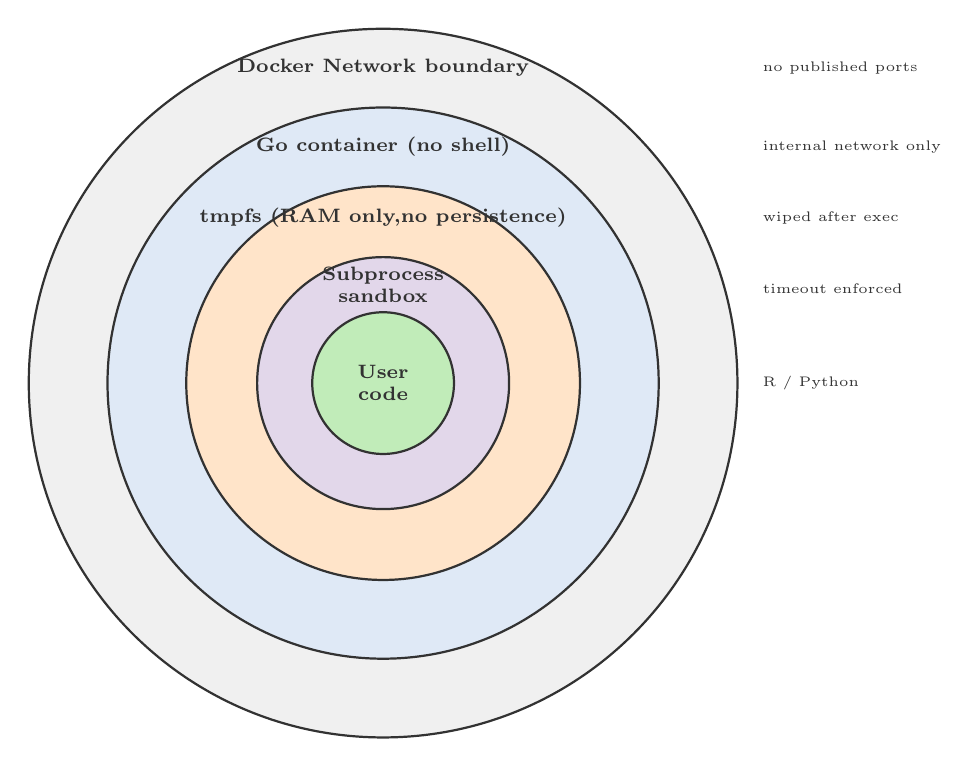
\begin{tikzpicture}
% Concentric circles (outermost first)
\fill[LGr!50, draw=DG, thick]   (0,0) circle (4.5cm);
\fill[LB!40,  draw=DG, thick]   (0,0) circle (3.5cm);
\fill[LO!40,  draw=DG, thick]   (0,0) circle (2.5cm);
\fill[LP!50,  draw=DG, thick]   (0,0) circle (1.6cm);
\fill[LG!60,  draw=DG, thick]   (0,0) circle (0.9cm);

% Labels
\node[font=\scriptsize\bfseries, text=DG] at (0, 4.0) {Docker Network boundary};
\node[font=\scriptsize\bfseries, text=DG] at (0, 3.0) {Go container (no shell)};
\node[font=\scriptsize\bfseries, text=DG] at (0, 2.1) {tmpfs (RAM only,\\no persistence)};
\node[font=\scriptsize\bfseries, text=DG, align=center] at (0, 1.25) {Subprocess\\sandbox};
\node[font=\scriptsize\bfseries, text=DG, align=center] at (0, 0)
  {User\\code};

% Side annotations
\node[font=\tiny, text=DG, anchor=west] at (4.7, 4.0) {no published ports};
\node[font=\tiny, text=DG, anchor=west] at (4.7, 3.0) {internal network only};
\node[font=\tiny, text=DG, anchor=west] at (4.7, 2.1) {wiped after exec};
\node[font=\tiny, text=DG, anchor=west] at (4.7, 1.2) {timeout enforced};
\node[font=\tiny, text=DG, anchor=west] at (4.7, 0.0) {R / Python};
\end{tikzpicture}
\caption{Security isolation concentric model for user-submitted R/Python
         execution. Code runs inside a RAM-only \texttt{tmpfs} ephemeral
         volume within a Go container on an internal Docker network,
         providing five isolation layers.}
\label{fig:security}
\end{figure}

% ╔══════════════════════════════════════════════════════════════════════════╗
% ║  FIG 22 — End-to-End Document Generation Timeline                       ║
% ╚══════════════════════════════════════════════════════════════════════════╝
\begin{figure}[h!]
\centering
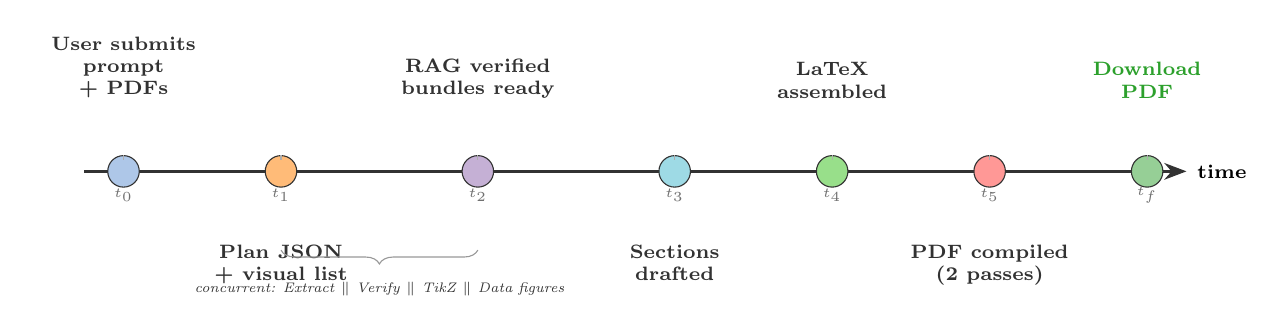
\begin{tikzpicture}[
  ev/.style={draw=DG, circle, fill=#1, minimum size=0.4cm, inner sep=0},
  lbl/.style={font=\scriptsize\bfseries, text=DG, align=center, text width=2.2cm},
  time/.style={font=\tiny, text=DG!70}
]
% Timeline axis
\draw[-{Stealth[length=8pt,width=6pt]}, very thick, draw=DG]
  (-6.5,0)--(7.5,0) node[right, font=\scriptsize\bfseries]{time};

% Events
\node[ev=LB]  (e1) at (-6,0)  {};
\node[ev=LO]  (e2) at (-4,0)  {};
\node[ev=LP]  (e3) at (-1.5,0){};
\node[ev=LT]  (e4) at (1.0,0) {};
\node[ev=LG]  (e5) at (3.0,0) {};
\node[ev=LR]  (e6) at (5.0,0) {};
\node[ev=CG!50](e7) at (7,0)  {};

% Labels above/below alternating
\node[lbl, above=0.6cm of e1] {User submits\\prompt + PDFs};
\node[lbl, below=0.6cm of e2] {Plan JSON\\+ visual list};
\node[lbl, above=0.6cm of e3] {RAG verified\\bundles ready};
\node[lbl, below=0.6cm of e4] {Sections\\drafted};
\node[lbl, above=0.6cm of e5] {LaTeX\\assembled};
\node[lbl, below=0.6cm of e6] {PDF compiled\\(2 passes)};
\node[lbl, above=0.6cm of e7, text=CG] {Download\\PDF};

% Time labels on axis
\node[time] at (-6,-0.3) {$t_0$};
\node[time] at (-4,-0.3) {$t_1$};
\node[time] at (-1.5,-0.3){$t_2$};
\node[time] at (1.0,-0.3) {$t_3$};
\node[time] at (3.0,-0.3) {$t_4$};
\node[time] at (5.0,-0.3) {$t_5$};
\node[time] at (7,-0.3) {$t_f$};

% Connector lines
\foreach \e in {e1,e2,e3,e4,e5,e6,e7}
  \draw[draw=DG!40, thin] (\e)--++(0,0.15);

% Parallel annotation
\draw[decorate, decoration={brace, amplitude=5pt, mirror}, draw=DG!50]
  (-4,-1.0)--(-1.5,-1.0)
  node[midway, below=8pt, font=\tiny\itshape, text=DG]
    {concurrent: Extract $\parallel$ Verify $\parallel$ TikZ $\parallel$ Data figures};
\end{tikzpicture}
\caption{End-to-end document generation timeline. Stages\,2, 2.3, 2.5, and
         2.7 execute concurrently over uploaded references; only Stage\,3
         drafting is sequential (for cross-section continuity).}
\label{fig:timeline}
\end{figure}

% ╔══════════════════════════════════════════════════════════════════════════╗
% ║  FIG 23 — Analytics Chart Taxonomy Grid                                 ║
% ╚══════════════════════════════════════════════════════════════════════════╝
\begin{figure}[h!]
\centering
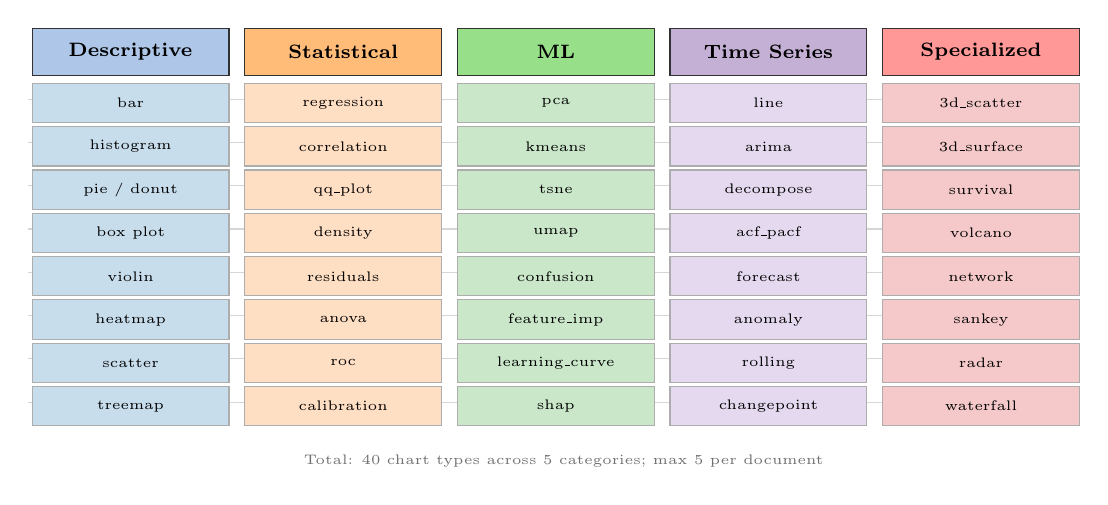
\begin{tikzpicture}[
  hdr/.style={draw=DG, fill=#1, minimum width=2.5cm, minimum height=0.6cm,
              align=center, font=\scriptsize\bfseries},
  cell/.style={draw=DG!40, fill=#1!25, minimum width=2.5cm, minimum height=0.5cm,
               align=center, font=\tiny}
]
% Column headers (chart categories)
\node[hdr=LB]  at (0,  0) {Descriptive};
\node[hdr=LO]  at (2.7,0) {Statistical};
\node[hdr=LG]  at (5.4,0) {ML};
\node[hdr=LP]  at (8.1,0) {Time Series};
\node[hdr=LR]  at (10.8,0){Specialized};

% Rows
\foreach \row/\y in {1/-0.65, 2/-1.2, 3/-1.75, 4/-2.3, 5/-2.85, 6/-3.4, 7/-3.95, 8/-4.5} {
  \draw[draw=DG!20, thin] (-1.3,\y+0.05)--(12.0,\y+0.05);
}

% Descriptive
\node[cell=CB] at (0,-0.65)  {bar};
\node[cell=CB] at (0,-1.2)   {histogram};
\node[cell=CB] at (0,-1.75)  {pie / donut};
\node[cell=CB] at (0,-2.3)   {box plot};
\node[cell=CB] at (0,-2.85)  {violin};
\node[cell=CB] at (0,-3.4)   {heatmap};
\node[cell=CB] at (0,-3.95)  {scatter};
\node[cell=CB] at (0,-4.5)   {treemap};

% Statistical
\node[cell=CO] at (2.7,-0.65){regression};
\node[cell=CO] at (2.7,-1.2) {correlation};
\node[cell=CO] at (2.7,-1.75){qq\_plot};
\node[cell=CO] at (2.7,-2.3) {density};
\node[cell=CO] at (2.7,-2.85){residuals};
\node[cell=CO] at (2.7,-3.4) {anova};
\node[cell=CO] at (2.7,-3.95){roc};
\node[cell=CO] at (2.7,-4.5) {calibration};

% ML
\node[cell=CG] at (5.4,-0.65){pca};
\node[cell=CG] at (5.4,-1.2) {kmeans};
\node[cell=CG] at (5.4,-1.75){tsne};
\node[cell=CG] at (5.4,-2.3) {umap};
\node[cell=CG] at (5.4,-2.85){confusion};
\node[cell=CG] at (5.4,-3.4) {feature\_imp};
\node[cell=CG] at (5.4,-3.95){learning\_curve};
\node[cell=CG] at (5.4,-4.5) {shap};

% Time series
\node[cell=CP] at (8.1,-0.65){line};
\node[cell=CP] at (8.1,-1.2) {arima};
\node[cell=CP] at (8.1,-1.75){decompose};
\node[cell=CP] at (8.1,-2.3) {acf\_pacf};
\node[cell=CP] at (8.1,-2.85){forecast};
\node[cell=CP] at (8.1,-3.4) {anomaly};
\node[cell=CP] at (8.1,-3.95){rolling};
\node[cell=CP] at (8.1,-4.5) {changepoint};

% Specialized
\node[cell=CR] at (10.8,-0.65){3d\_scatter};
\node[cell=CR] at (10.8,-1.2) {3d\_surface};
\node[cell=CR] at (10.8,-1.75){survival};
\node[cell=CR] at (10.8,-2.3) {volcano};
\node[cell=CR] at (10.8,-2.85){network};
\node[cell=CR] at (10.8,-3.4) {sankey};
\node[cell=CR] at (10.8,-3.95){radar};
\node[cell=CR] at (10.8,-4.5) {waterfall};

\node[font=\tiny, text=DG!70] at (5.5,-5.2)
  {Total: 40 chart types across 5 categories; max 5 per document};
\end{tikzpicture}
\caption{Analytics pipeline chart taxonomy: 40 chart types across five
         semantic categories. The LLM selects up to five plans per document;
         column existence is validated before code generation.}
\label{fig:charttax}
\end{figure}

% ╔══════════════════════════════════════════════════════════════════════════╗
% ║  FIG 24 — Template Resolution Priority Chain                            ║
% ╚══════════════════════════════════════════════════════════════════════════╝
\begin{figure}[h!]
\centering
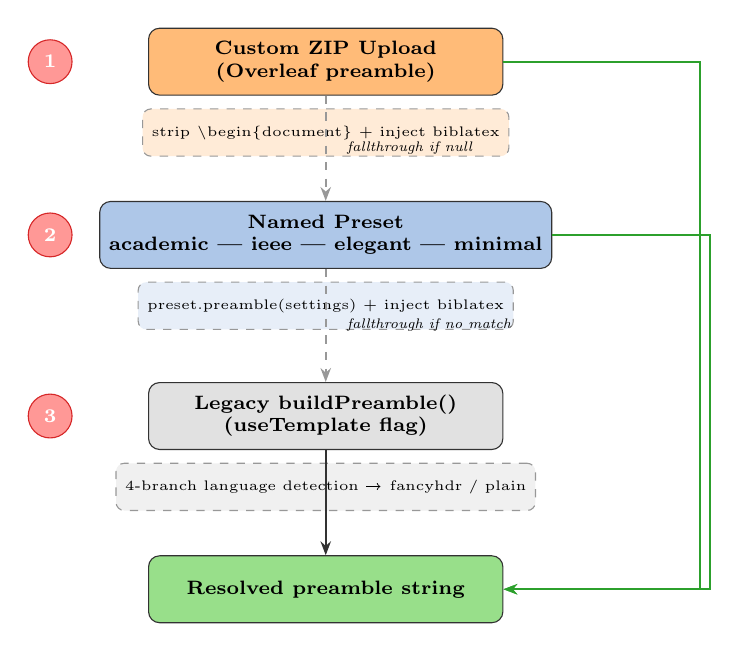
\begin{tikzpicture}[
  prio/.style={draw=DG, rounded corners=4pt, fill=#1,
               minimum width=4.5cm, minimum height=0.85cm,
               align=center, font=\scriptsize\bfseries},
  sub/.style={draw=DG!50, dashed, rounded corners=3pt, fill=#1,
              minimum width=3.8cm, minimum height=0.6cm,
              align=center, font=\tiny},
  arr/.style={-{Stealth[length=5pt]}, thick, draw=DG},
  badge/.style={draw=CR, circle, fill=LR, minimum size=0.55cm,
                font=\scriptsize\bfseries, text=white}
]
\node[badge] (b1) at (-3.5, 3.0) {1};
\node[prio=LO] (custom) at (0, 3.0)
  {Custom ZIP Upload\\(Overleaf preamble)};
\node[sub=LO!30] at (0, 2.1) {strip \textbackslash begin\{document\} + inject biblatex};

\node[badge] (b2) at (-3.5, 0.8) {2};
\node[prio=LB] (preset) at (0, 0.8)
  {Named Preset\\academic | ieee | elegant | minimal};
\node[sub=LB!30] at (0,-0.1) {preset.preamble(settings) + inject biblatex};

\node[badge] (b3) at (-3.5,-1.5) {3};
\node[prio=LGr] (legacy) at (0,-1.5)
  {Legacy buildPreamble()\\(useTemplate flag)};
\node[sub=LGr!50] at (0,-2.4) {4-branch language detection → fancyhdr / plain};

% Priority arrows
\draw[arr, dashed, draw=DG!50] (custom)--(preset)
  node[midway, right=4pt, font=\tiny\itshape]{fallthrough if null};
\draw[arr, dashed, draw=DG!50] (preset)--(legacy)
  node[midway, right=4pt, font=\tiny\itshape]{fallthrough if no match};

% Output
\node[prio=LG, minimum width=4.5cm] (out) at (0,-3.7)
  {Resolved preamble string};
\draw[arr] (legacy)--(out);
\draw[arr, CG] (custom.east)--++(2.5,0)|-(out.east);
\draw[arr, CG] (preset.east)--++(2.0,0)|-(out.east);
\end{tikzpicture}
\caption{Template resolution priority chain (\texttt{resolveTemplate()}). Custom
         Overleaf ZIP uploads take highest priority; named presets override the
         legacy flag-based builder; all paths inject \texttt{biblatex} when
         references are enabled.}
\label{fig:template}
\end{figure}

% ╔══════════════════════════════════════════════════════════════════════════╗
% ║  FIG 25 — Knowledge Base Injection Architecture                         ║
% ╚══════════════════════════════════════════════════════════════════════════╝
\begin{figure}[h!]
\centering
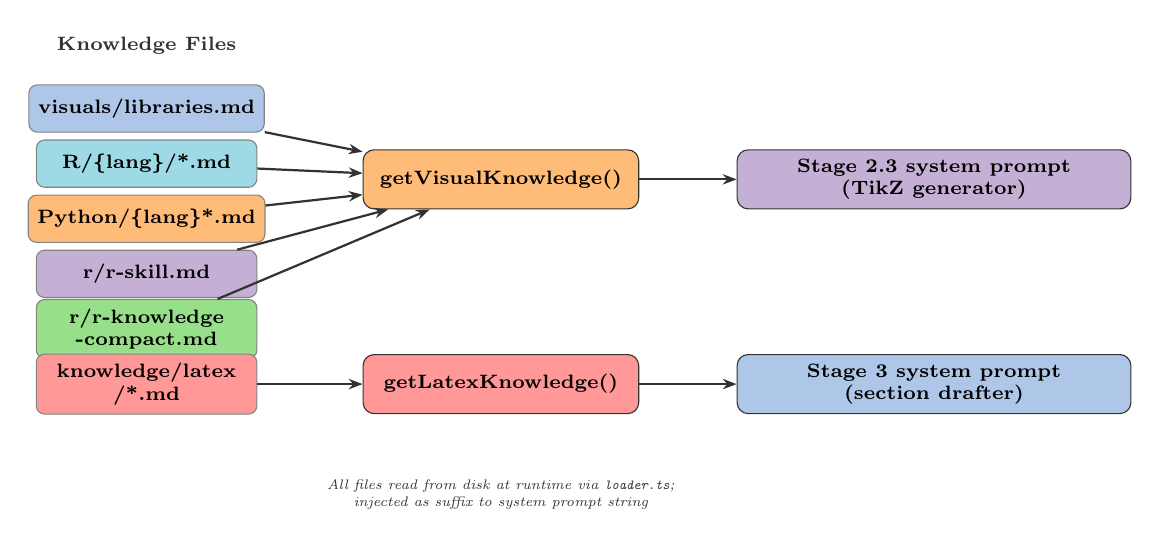
\begin{tikzpicture}[
  src/.style={draw=DG!60, fill=#1, rounded corners=3pt,
              minimum width=2.8cm, minimum height=0.6cm,
              align=center, font=\scriptsize\bfseries},
  fn/.style={draw=DG, fill=#1, rounded corners=4pt,
             minimum width=3.5cm, minimum height=0.75cm,
             align=center, font=\scriptsize\bfseries},
  tgt/.style={draw=DG, fill=#1, rounded corners=4pt,
              minimum width=5cm, minimum height=0.75cm,
              align=center, font=\scriptsize\bfseries},
  arr/.style={-{Stealth[length=5pt]}, thick, draw=DG}
]
% Knowledge sources
\node[font=\scriptsize\bfseries, text=DG] at (-4.5, 3.5) {Knowledge Files};
\node[src=LB]  (lib)  at (-4.5, 2.7) {visuals/libraries.md};
\node[src=LT]  (rmd)  at (-4.5, 2.0) {R/\{lang\}/*.md};
\node[src=LO]  (pymd) at (-4.5, 1.3) {Python/\{lang\}*.md};
\node[src=LP]  (rsk)  at (-4.5, 0.6) {r/r-skill.md};
\node[src=LG]  (rkn)  at (-4.5,-0.1) {r/r-knowledge\\-compact.md};
\node[src=LR]  (ltx)  at (-4.5,-0.8) {knowledge/latex\\/*.md};

% Loader functions
\node[fn=LO] (gvk) at (0, 1.8) {getVisualKnowledge()};
\node[fn=LR] (glk) at (0,-0.8) {getLatexKnowledge()};

% Injection targets
\node[tgt=LP] (s23sys) at (5.5, 1.8) {Stage 2.3 system prompt\\(TikZ generator)};
\node[tgt=LB] (s3sys)  at (5.5,-0.8) {Stage 3 system prompt\\(section drafter)};

% Arrows
\draw[arr] (lib)--(gvk);
\draw[arr] (rmd)--(gvk);
\draw[arr] (pymd)--(gvk);
\draw[arr] (rsk)--(gvk);
\draw[arr] (rkn)--(gvk);
\draw[arr] (ltx)--(glk);
\draw[arr] (gvk)--(s23sys);
\draw[arr] (glk)--(s3sys);

\node[font=\tiny\itshape, text=DG, align=center] at (0,-2.2)
  {All files read from disk at runtime via \texttt{loader.ts};\\
   injected as suffix to system prompt string};
\end{tikzpicture}
\caption{Knowledge base injection architecture. Domain-specific Markdown files
         covering TikZ libraries, R/Python analytics, and LaTeX conventions are
         loaded at runtime and appended to the respective stage system prompts,
         decoupling knowledge management from code.}
\label{fig:knowledge}
\end{figure}

\end{document}
